%%% -*-LaTeX-*-

\chapter{Data-Driven Correlation Analysis Between Observed 3D Fatigue\allowbreak-Crack Path and Computed Fields from High-Fidelity, Crystal\allowbreak-Plasticity, Finite-Element Simulations}

As described in the previous chapter, a better representation of the data is needed in order to facilitate a more exhaustive investigation of the features related to crack growth.  The inspiration for this representation is the way in which images are typically depicted, namely by a 2-dimensional grid of pixels, where each pixel contains a vector of integers corresponding to an element of a color space.  The motivation for using images as an inspiration is based on the ability of convolutional neural networks (CNNs) to learn relevant features given such a representation.  CNNs can easily extend to 3-dimensions, so all spatial information can be retained by simply converting the 3-dimensional microstructure into a 3-dimensional grid with $1 \mu m$ spacing.  All that remains is to choose which values will fill the vector at each grid point.  This chapter includes content from a paper published in the Journal of the Minerals, Metals, and Materials Society (JOM) in 2018 \cite{pierson2018}.  It explores using correlation between the values of various micromechanical field variables and distance to crack surface as a method of choosing the values for these vectors.  The supplementary materials referenced in this chapter are also included. \footnote{Reprinted by permission from [Springer Nature]: [The Minerals, Metals, and Materials Society] [JOM] \cite{pierson2018} (Data-Driven Correlation Analysis Between Observed 3D Fatigue-Crack Path and Computed Fields from High-Fidelity, Crystal-Plasticity, Finite-Element Simulations, K. Pierson, A. Spear, J. Hochhalter), \copyright\ (2018)}

%\setupuuchapterbib

%\uudummysection    {Introduction}                                                         {1}

%\uudummysection    {Materials and Methods}                                                {2}
%\uudummysubsection {Experimental Measurements and Mesh Generation from Prior Work}        {2}
%\index{X-ray computed tomography}
%\index{Near-field high-energy X-ray diffraction microscopy}
%\uudummysubsection {Numerical Simulation of Cyclic Loading Applied to Uncracked Specimen} {2}

%\uudummyfigure     {Volume and crack surface reconstructions}                             {3}
%\uudummyfigure     {Applied boundary conditions}                                          {3}

%\uudummytable      {Calibrated material parameters}                                       {4}
%\uudummysubsection {Convergence of Cyclic Field Variables}                                {4}
%\uudummysubsection {Correlation Analysis}                                                 {4}
%\index{Pearson moment-product correlation}

%\uudummyfigure     {Convergence of $\Delta \sigma$ values}                                {5}
%\uudummyfigure     {Cyclic micromechanical Taylor factor}                                 {5}

%\uudummysection    {Results and Discussion}                                               {6}
%\uudummyfigure     {Filtered points for correlation analysis}                             {6}

%\uudummyfigure     {Algorithm flowchart}                                                  {7}
%\uudummyfigure     {Fracture surface correlations}                                        {7}

%\uudummyfigure     {Offset fracture surface correlations}                                 {8}
%\uudummysection    {Conclusion}                                                           {8}

%\uudummysection    {Acknowledgements}                                                     {9}
%\uudummysection    {Electronic Supplementary Material}                                    {9}
%\uudummysection    {References}                                                           {9}

%\includepdf [
%                   pages = -,                        % want all document pages
%                   scale = 0.91,                     % adjust to fit thesis page box
%                   pagecommand = {\pagestyle{plain}} % bare page numbers
%            ]{data-driven-correlation.pdf}

A systematic correlation analysis is performed between simulated micromechanical fields in an uncracked polycrystal and the known path of an eventual fatigue-crack surface based on experimental observation. A concurrent multi-scale finite-element simulation of cyclic loading is performed using a high-fidelity representation of grain structure obtained from near-field high-energy X-ray diffraction microscopy measurements. An algorithm is developed to parameterize and systematically correlate the 3D micromechanical fields from simulation with the 3D fatigue-failure surface from experiment. As a comparison, correlation coefficients are also computed between the micromechanical fields and hypothetical, alternative surfaces. Correlation of the fields with hypothetical surfaces is found to be consistently weaker than correlation with the known crack surface, suggesting that the micromechanical fields of the cyclically loaded, uncracked microstructure might provide some degree of predictiveness for microstructurally small fatigue-crack path. Although, the extent of such predictiveness remains to be tested. In general, gradients of the field variables exhibit stronger correlations with crack path than the field variables, themselves. Results from the data-driven approach implemented here can be leveraged in future model development for the prediction of fatigue-failure surfaces (for example, to facilitate univariate feature selection required by convolution-based models).

\section{Introduction}
% Motivation for fatigue modeling of MSFCs
Microstructural features play a governing role in the initiation and early stages of fatigue-crack growth. Variation in those features leads directly to variation in the paths and growth rates of microstructurally small cracks and, consequently, to scatter among fatigue lifetimes of structural components. Modeling this variability is critical given that most of the service life of fatigue-critical components can be consumed by initiation and growth of microstructure-sensitive cracks. Yet, these early stages of fatigue-crack evolution are difficult to model because of the complex dependence on a broad scope of microstructural features and the tendency to exceed propagation rates of long cracks with equivalent nominal stress intensity factors \cite{Ritchie_1986}. The reader is directed to Ref.~\cite{Murty_2017} for an encompassing review of the metallographic aspects of microstructural heterogeneities and their role in fatigue cracking. Similarly, a review of the micromechanical descriptions of the effect of microstructural heterogeneities is given in Ref.~\cite{Mughrabi_2014}.

%Early attempts at modeling microstructure-performance variability
%Empirical approaches are not the answer
Empirically based fatigue-life models were developed to link variability in fatigue life to microstructural features that were directly observable and quantifiable. Early examples of these approaches, which are overviewed in Refs.~\cite{Murakami_1994, Fatemi_1998, Hussain_1997}, based fatigue models on microstructural characteristics such as inclusion size, shape, and location \cite{Laz_1998, Brockenbrough_1994, Przystupa_1997}. While empirical approaches have provided foundational knowledge regarding microstructural effects on fatigue performance, the resulting correlations and applicability of the developed models are valid only within the domain of the measured data and experimental parameters (e.g., boundary conditions, cyclic-load ratio, etc.). The formative works of Wei and Harlow \cite{Wei_2005, Harlow_2009} clearly illustrate the need to use experimentation to discover and formulate hypotheses regarding the micromechanics at hand, not to fit empirical parameters.  

%Modeling micromechanisms
Over the past two decades, there has been a shift toward computationally modeling microstructural features to investigate their impact on fatigue-crack initiation and early propagation. Such efforts typically use crystal-plasticity formulations to incorporate elastic and plastic anisotropy and either statistically-representative or directly replicated microstructural domains to capture heterogeneities. For example, Bozek et al.~\cite{Bozek_2008} simulated the effect of cyclic loading on cracking of second-phase particles. Subsequently, Hochhalter et al.~\cite{hochhalter2010geometric, Hochhalter_2011} used fatigue indicator parameters to predict which cracks would extend beyond those cracked particles.  Twin boundary crack initiation sites, and their dependence on local microstructure, was presented by Yeratapally et al. \cite{Yeratapally_2016}.  Fatigue indicator parameters were used by Musinski et al. \cite{Musinski_2016} and Castelluccio et al. \cite{Castelluccio_2016} to develop models for the subsequent propagation of cracks across a polycrystal. An encompassing study of the fatigue indicator parameters proposed to date is provided by Rovinelli et al. \cite{Rovinelli_2017}. These studies represent a small sampling of high-fidelity, microstructure-sensitive fatigue modeling, and a more complete review can be found in Refs.~\cite{Sangid_2013, McDowell_2010, Castelluccio_2014, Christ_2014}.  

%Holistic 3DMS movement
Advancements in these micromechanical modeling methods are being closely coupled with volumetric interrogation methods.  This coupled approach provides a capability whereby parameters that cannot be measured directly can be computed in a simulation that serves to replicate the particular microstructure of the specimen. Spear et al.~\cite{spear2016} used near-field high-energy X-ray diffraction (HEDM) to measure grain morphology in a sample of Al 6061-T6. These data were then used to generate a finite-element model, which replicated the as-measured grain structure and crack morphology. Rovinelli et al.~\cite{Rovinelli_2017} used diffraction contrast and phase contrast tomography to measure microstructure morphology and evolved crack faces in a near-$\beta$ Ti alloy.  Those data were used to generate a 3D FFT simulation with crystal plasticity.  Bayesian networks were then used to analyze correlation between the proposed short-crack driving forces and experimental observations. 

As highlighted by the aforementioned studies, integrating X-ray-based measurement methods with high-fidelity simulation tools is providing a promising new approach to developing models for short-crack propagation \cite{Turner_2017}. New focus is on the efficient processing of these data (which can be quite large and complex) to extract useful information using data-driven approaches. In light of this, the objective of this paper is to describe a systematic, data-driven, correlation analysis between computed micromechanical fields of an uncracked, cyclically loaded 3D polycrystal and the known path of a 3D fatigue-failure surface based on direct observation from prior experimental measurements.

\section{Materials and methods}\label{methods}
\subsection{Experimental measurements and mesh generation from prior work} \label{prior_work}
The data used in this work are derived from experimental measurements \cite{spear2014} of 3D fatigue crack propagation within a grain-mapped volume of an Al-Mg-Si alloy. In that work, a naturally nucleated fatigue crack was propagated to failure under cyclic loading. The material volume above and below the failure surface was characterized post-mortem using X-ray computed tomography and near-field HEDM. The former provided a high-resolution reconstruction of the failure surface, and the latter provided 3D grain maps adjacent to the failure surfaces, which can be seen in Fig.~\ref{fig:exp_data_actamat}. Of the entire measured crack surface, 31.8\% was found to be approximately normal (within 20\degrees) to the global loading direction. Additionally, 41\% and 59\% of the entire crack surface was deemed to be intergranular and transgranular, respectively, with the transgranular crack surface occurring along a wide variety of crystallographic planes.

The two halves of post-mortem data were then virtually merged to generate a conformal finite-element mesh that represents explicitly and with high fidelity the internal grain boundaries and incremental crack surfaces measured from experiment, which is detailed in Ref. \cite{spear2016}. In this work, the conformal finite-element mesh representing the uncracked microstructure is used to obtain computed micromechanical fields, which are correlated with the reconstructed failure surface. Fig.~\ref{fig:exp_data_actamat} summarizes the prior relevant work.
\begin{figure}[b]
  \centering
    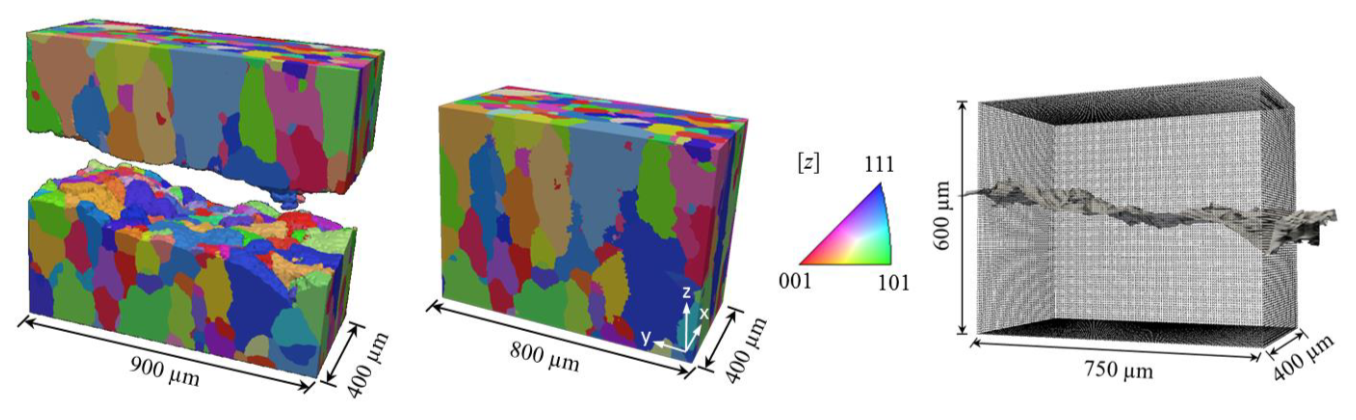
\includegraphics[width=\hsize]{exp_data_actamat}
    \caption{Post-mortem reconstructions from an Al-Mg-Si alloy fatigue specimen based on near-field HEDM. (a). Approximation of uncracked volume (b) and reconstructed fatigue-failure surface from X-ray CT (c). The reference coordinate system is shown on the uncracked microstructural volume. Adapted with permission from Refs.\ \cite{spear2016} and \cite{spear2014}.}
    \label{fig:exp_data_actamat}
\end{figure}

\subsection{Numerical simulation of cyclic loading applied to uncracked specimen} \label{simulation}
A concurrent multi-scale finite-element model is used to simulate cyclically applied displacement on the fatigue specimen tested in previous work \cite{spear2016}. The previously generated mesh from Ref. \cite{spear2016} consists of a local, polycrystalline region representing the uncracked microstructure and a global region representing the geometry of the fatigue specimen, shown in Fig.~\ref{fig:mesh_and_cycle_count}. A mesh convergence study, detailed in Ref. \cite{spear2014numerical}, was carried out to ensure that both the global force-displacement response and local stresses, strains, and accumulated slip along an arbitrary query path through the polycrystalline domain are sufficiently converged. The converged, multi-scale mesh comprises 11.86M quadratic tetrahedral elements.
\begin{figure}[b]
  \centering
    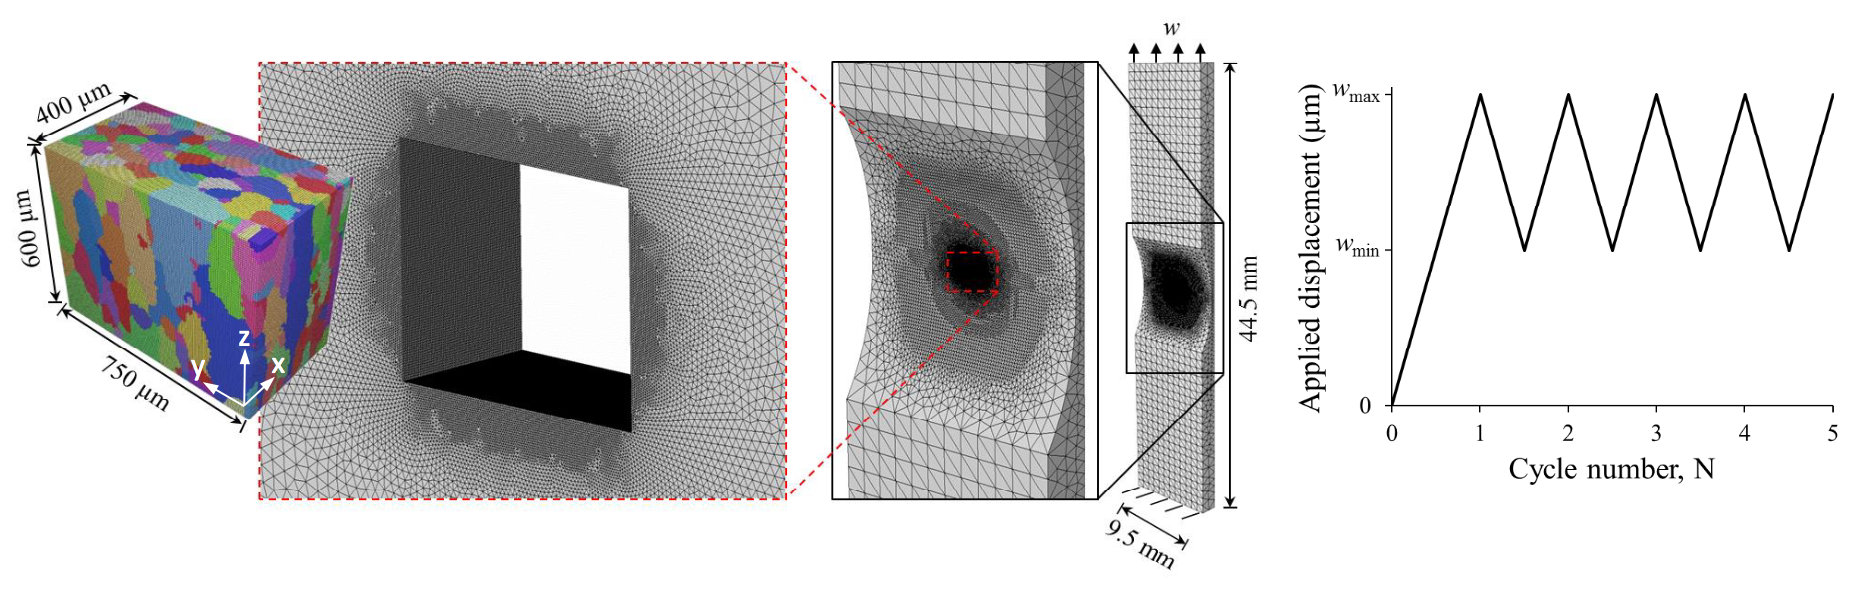
\includegraphics[width=\hsize]{mesh_and_cycle_count}
    \caption{Concurrent multi-scale finite-element mesh and applied boundary conditions. The reference coordinate system is shown on the uncracked microstructural volume. Adapted with permission from Ref.\ \cite{spear2016}.}
    \label{fig:mesh_and_cycle_count}
\end{figure}

A crystal, elasto-viscoplastic, constitutive model based on the implementation by Matous and Maniatty \cite{Matouvs2004} is applied to the polycrystalline domain, and a J2-plasticity model is applied to the global domain. Both models are calibrated to ensure that the nominal (averaged) stress-strain behavior matches experimental data for the same material and that the simulated macroscopic-strain fields in the notch region match those from digital image correlation measurements, which are described elsewhere \cite{spear2014numerical}. The crystal, elasto-viscoplastic, constitutive model is capable of predicting inhomogeneous deformation and stress fields that arise at the mesoscale as a result of interactions among discrete grains. In the model, plastic deformation is manifested by slip evolution on 12 octahedral slip systems ($\{111\}<110>$). All elements within the polycrystalline domain are assigned the same material properties; however, each element is assigned a crystal orientation based on the grain to which that element belongs. The crystal orientations are derived directly from the near-field HEDM measurements described above. The calibrated parameters for both constitutive models are provided in Table 3.1. Properties for the J2-plasticity model include the elastic modulus ($E$), Poisson’s ratio ($\nu$), yield strength ($\sigma_y$), and hardening modulus ($h'$). Properties for the crystal-plasticity model include a reference slip rate ($\dot{\gamma}_0$), a hardening rate-sensitivity parameter ($m$), a hardening-rate parameter ($G_0$), and initial hardness ($g_0$).

\begin{table}[b]
  \small
  \centering
  \label{table:material_parameters}
  \caption{Calibrated material parameters.}
  \begin{tabularx}{\textwidth}{|c *{10}{|Y}|}
    \hline
    \multicolumn{4}{|c|}{J2-plasticity model} &
    \multicolumn{4}{c|}{Crystal plasticity model} \\
    \hline
    $E(MPa)$ & $\nu$ & $\sigma_y(MPa)$ & $h'(MPa)$ & $\dot{\gamma_0}(s^{-1})$ & $m$ & $G_0(MPa)$ & $g_0(MPa)$ \\
    \hline
    70326 & 0.33 & 206.5 & 1200 & 0.05 & 0.0049 & 150.0 & 95.5 \\
    \hline
  \end{tabularx}
\end{table}

Boundary conditions are applied to replicate constraints and loading applied in the actual experiment. Namely, the grip ends of the specimen are constrained from displacing in the $x$ and $y$ directions. The lower grip end is further constrained from displacing in the $z$ direction. The upper grip end is subjected to vertical displacement, $w$, which cycles between $w_{max}=65$ $\mu$m and $w_{min}=38$ $\mu$m. The values for applied displacement are selected to reproduce the applied loading from experiment, detailed in Ref. \cite{spear2014}. 

Numerical simulation is performed using the parallelized finite-element code ScIFEN \cite{warner2016scalable}. In total, five load cycles are simulated. The following list summarizes all local variables that are recorded for the entire polycrystalline domain at the beginning and end of each simulated load cycle.

\begin{itemize}[noitemsep]
  \renewcommand\labelitemi{}
  \item $D_1$ \tabto{1.5cm} = \tabto{2cm} Maximum value of accumulated slip among the 12 octahedral slip systems 
  \item $D_2$ \tabto{1.5cm} = \tabto{2cm} Maximum value of total accumulated slip over each slip plane
  \item $D_3$ \tabto{1.5cm} = \tabto{2cm} Accumulated slip summed over all slip systems
  \item $D_4$ \tabto{1.5cm} = \tabto{2cm} Maximum value of energy dissipated on a given slip plane during plastic deformation
  \item $D_5$ \tabto{1.5cm} = \tabto{2cm} Modified Fatemi-Socie parameter
  \item $\overline{\epsilon}$ \tabto{1.5cm} = \tabto{2cm} Symmetric strain tensor composed of $\epsilon_{xx}$, $\epsilon_{yy}$, $\epsilon_{zz}$, $\epsilon_{xy}$, $\epsilon_{xz}$, and $\epsilon_{yz}$
  \item $\epsilon_{1}$ \tabto{1.5cm} = \tabto{2cm} Principal eigenvalue of the strain tensor
  \item $\epsilon_{vm}$ \tabto{1.5cm} = \tabto{2cm} Von Mises strain
  \item $\overline{\sigma}$ \tabto{1.5cm} = \tabto{2cm} Symmetric stress tensor composed of $\sigma_{xx}$, $\sigma_{yy}$, $\sigma_{zz}$, $\sigma_{xy}$, $\sigma_{xz}$, and $\sigma_{yz}$
  \item $\sigma_{1}$ \tabto{1.5cm} = \tabto{2cm} Principal eigenvalue of the stress tensor
  \item $\sigma_{vm}$ \tabto{1.5cm} = \tabto{2cm} Von Mises stress
  \item $M^{micro}$ \tabto{1.5cm} = \tabto{2cm} Micromechanical Taylor factor \cite{raabe2001}
\end{itemize}

The variables $D_{1...5}$ represent slip-based damage metrics described by Hochhalter, et al. \cite{hochhalter2010geometric} and implemented within the ScIFEN framework. Additionally, micromechanical Taylor factor, $M^{micro}$, is computed throughout the polycrystalline domain based on the work of Raabe et al. \cite{raabe2001}, as shown in Equation~\ref{taylor_factor}.

\begin{equation}
\label{taylor_factor}
M^{micro} = \frac{D_3}{\epsilon_{vm}}.
\end{equation}

In Equation~\ref{taylor_factor}, $D_3$ is the summation over all $N_s$ slip systems of the slip accumulated on each slip system, $\alpha$, throughout cyclic loading:
\begin{equation}\label{D3}
D_3 = \sum_{\alpha=0}^{N_s}{\int_0^t {|\dot{\gamma}^{\alpha}|}dt},
\end{equation}
where $\dot{\gamma}^{\alpha}$ is the slip rate on a given slip system. The term $\epsilon_{vm}$ represents the local von Mises equivalent strain, which is computed as:
\begin{equation}\label{vonmises}
\epsilon_{vm} = \sqrt{\frac{2}{3} \overline{\epsilon} : \overline{\epsilon}}.
\end{equation}

The variables in the above list, along with the cyclic changes in those variables, are included in the systematic correlation analysis.

\subsection{Convergence of cyclic field variables}\label{convergence}
The convergence of field variables is assessed by considering the change in each variable throughout the entire polycrystalline domain as a function of cycle count. For any given variable, $\lambda$, its cyclic value is computed at each point in the model based on the change in that variable between minimum to maximum displacement over a given loading cycle. The change in each cyclic value is also computed between successive loading cycles. In other words, at each point in the model, and for all variables in a given cycle, $N$:
\begin{equation}\label{deltas}
\Delta \lambda_N = \lambda_{w_{max}, N} - \lambda_{w_{min}, N}\end{equation}
\begin{equation} \Delta^2 \lambda_N = \Delta \lambda_N - \Delta \lambda_{N-1}. \end{equation}

Fig.~\ref{fig:convergence} illustrates the convergence of $\Delta \sigma_{zz}$ and a visualization of $\Delta ^2 \sigma_{zz}$ approaching zero (similar convergence is verified for all variables). Convergence of the cyclic field variables implies that the results taken from the fifth loading cycle sufficiently represent the state of the polycrystalline domain to perform a meaningful correlation study.
\begin{figure}[b]
  \centering
    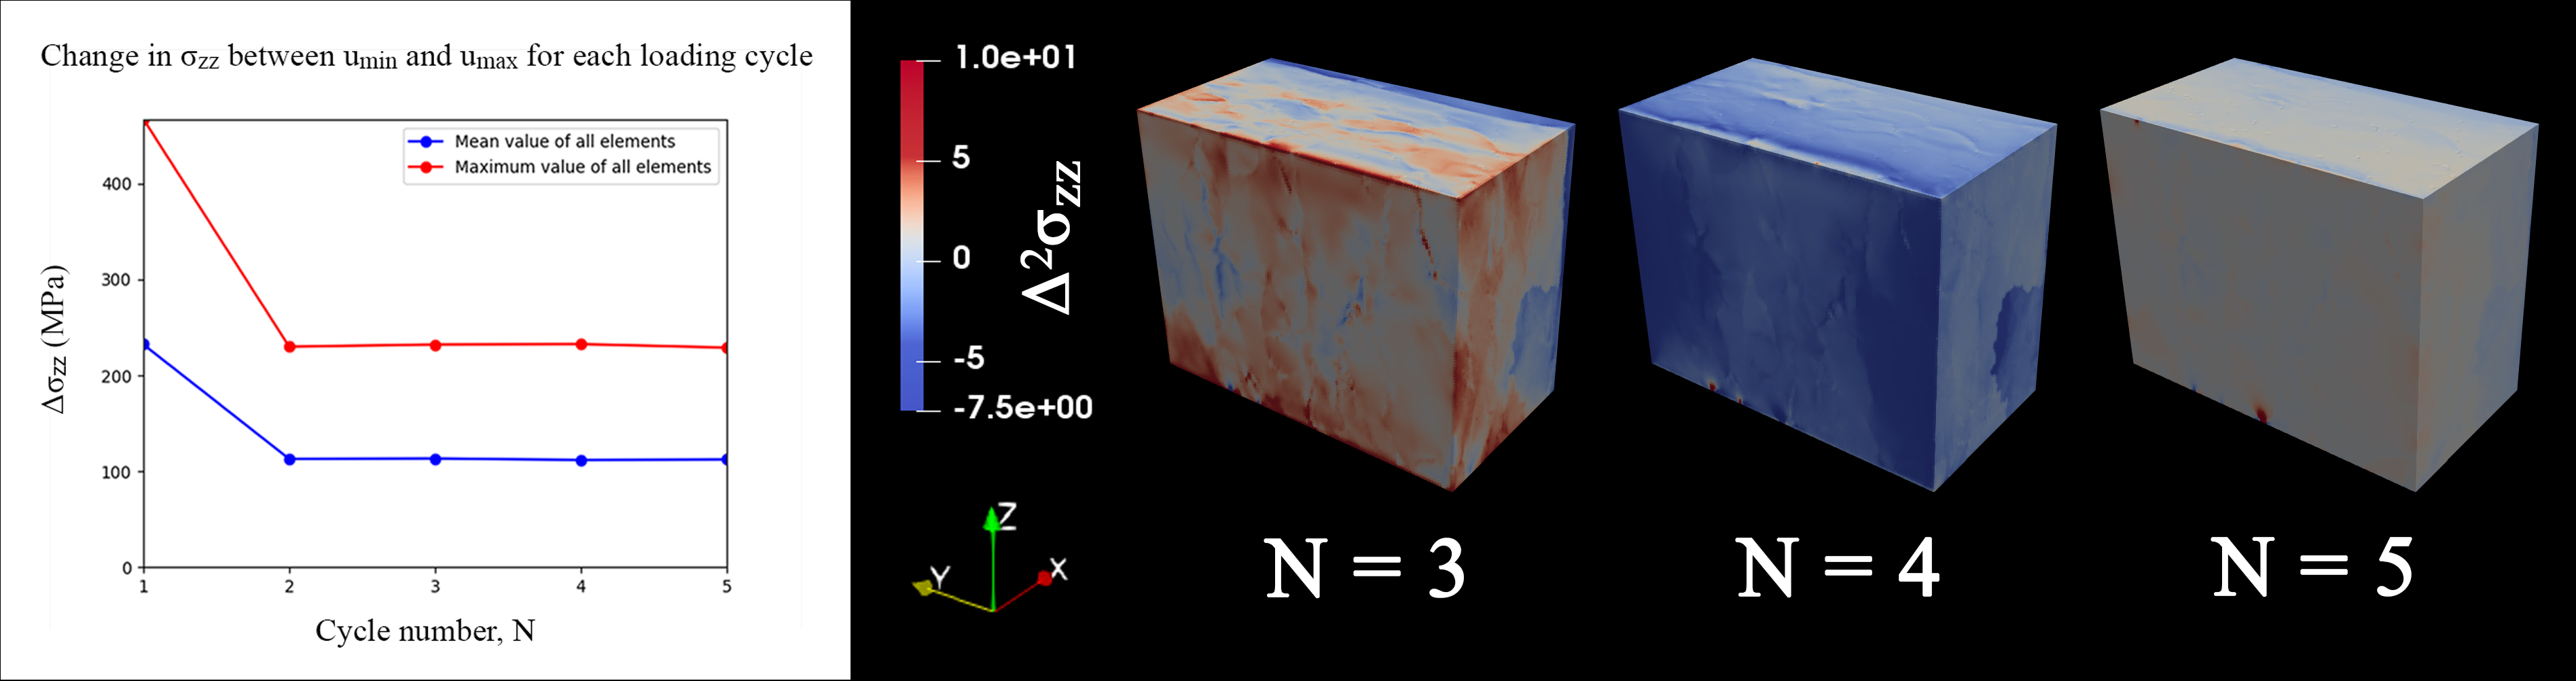
\includegraphics[width=\hsize]{convergence}
    \caption{Convergence of $\Delta \sigma_{zz}$ and $\Delta ^2 \sigma_{zz}$ (MPa) during cyclic loading.}
    \label{fig:convergence}
\end{figure}
 
\subsection{Correlation analysis}\label{correlation_analysis}
The finite-element results are first converted to a format amenable to performing the correlation analysis. Results associated with the fifth loading cycle are subsampled from the unstructured finite-element mesh onto a $383 \times 750 \times 600$ $\mu m^3$ grid with 1 $\mu$m spacing between points. This is done for all field variables, producing a scalar-valued grid for each variable, $\lambda$, corresponding to peak load, and for each cyclic value, $\Delta\lambda$.

Additionally, the spatial gradients of every $\lambda$ and $\Delta\lambda$ variable are calculated and included in the correlation analysis. Here, the gradients of $\lambda$ and $\Delta\lambda$ at each point in the model are computed based on finite differences in the $y$ and $z$ directions (reminiscent of 2D image slices through the volume) using $h$ = 3 $\mu m$ spacing\footnote{Values of 1 $\mu m$ and 3 $\mu m$ were considered for $h$, with the latter being equal to half the size of the discretization for the quadratic finite-element mesh. Ultimately, $h$ = 3 $\mu m$ was found to provide stronger correlations.}, after which the $L_2$ norm is taken to produce a scalar value. In the following equations, subscripts indicate the grid coordinates of a given point.
\begin{equation}
\frac{d\lambda_{x, y, z}}{dy} = \frac{\lambda_{x, y+h, z} - \lambda_{x, y-h, z}}{2h}, \quad 
\frac{d\lambda_{x, y, z}}{dz} = \frac{\lambda_{x, y, z+h} - \lambda_{x, y, z-h}}{2h}  \end{equation}

The next step is to represent the 3D crack surface, which was previously reconstructed from post-mortem X-ray CT data and aligned with the uncracked microstructural domain, as a 2D grid of elevation values. This is accomplished by initializing a $383 \times 750$ $\mu m^2$ grid with 1~$\mu$m spacing between points, and then assigning to each point an interpolated value of the corresponding $z$ coordinate of the crack surface, resulting in a height-map. The interpolation method is an inverse bilinear interpolation. For a given point in the $x-y$ grid plane, the corresponding height-map value of the crack surface is used to identify neighboring points in the 3D scalar-valued grids. 

In total, there are 88 scalar-valued grids to consider in the correlation analysis:~one for each field variable, $\lambda$, listed in Section~\ref{simulation}; one for each cyclic variable, $\Delta \lambda$; and one for the gradient values of both $\lambda$ and $\Delta \lambda$. Each grid consists of $383 \times 750 \times 600 = 1.724\times 10^{9}$ data points derived from high-fidelity numerical simulation of the uncracked microstructure. There are an additional $383 \times 750 = 2.87\times 10^{5}$ data points derived from the experimentally observed fatigue-failure surface.

Using this as input data, the goal of the algorithm implemented here is to determine -- with minimal prior assumptions -- which micromechanical field variables are correlated with fatigue-crack path. The method chosen here is to compute the correlation between the value of a given variable at a particular point in the microstructure and its vertical distance to the crack surface. Only a local neighborhood around the crack surface is considered, i.e. a region into which the crack could plausibly have grown from any given configuration. The value of $L$ was systematically varied, and ultimately a value of $L=25~\mu$m (approximately 25\% of the average grain diameter) above and below the crack surface is selected to optimize the correlation results. This value is used in all correlation analyses described throughout this paper. The definition of $L$ is shown in Fig.~\ref{fig:grid} for a slice and subsection of the grid defined for $\Delta M^{micro}$. The grid points are shown in black with a spacing of $1~\mu$m, and the finite-element results obtained using an unstructured mesh are shown in the background. The trace of the actual crack surface is superimposed for reference.  
\begin{figure}[b]
  \centering
    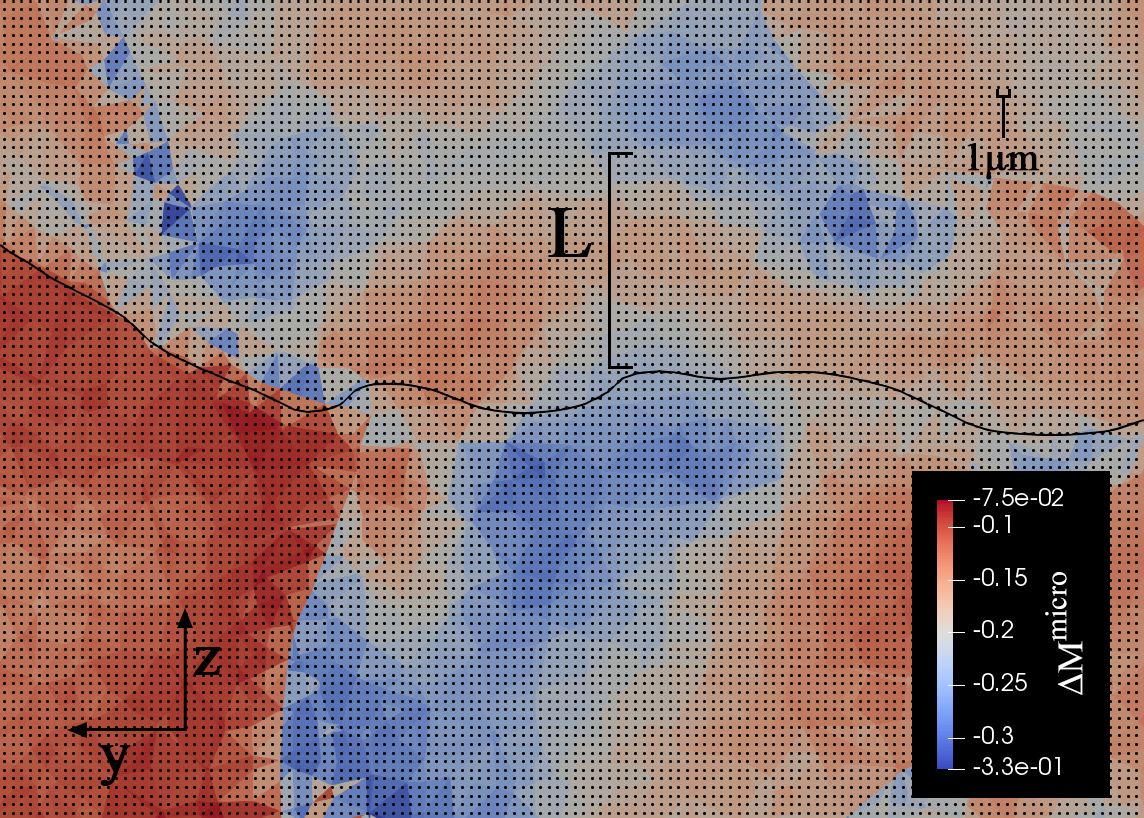
\includegraphics[width=0.5\hsize]{grid}
    \caption{Cyclic micromechanical Taylor factor computed for the uncracked polycrystal, shown at a particular slice through the volume. Superimposed is the trace of the actual crack surface from X-ray CT imaging. Also superimposed is the grid used for correlation analysis. The neighborhood of influence is defined by the distance $L$ above and below the crack surface.}
    \label{fig:grid}
\end{figure}

Of this subset of points within $L$ of the surface, only regions where the gradient of a given field variable is sufficiently high are considered. This filter is implemented due to the propensity of some variables to exhibit near-zero change within the neighborhood, $L$. In such cases, the correlation of that variable with distance to crack surface does not add value to the analysis. In order for a gradient of a variable to be considered sufficiently high, it must be at least $t\%$ of its value at the same point. Here, $t$ is determined independently for each variable by finding the value of $t$ that maximizes the correlation of that variable, while still retaining at least $10\%$ of the total crack surface (see Fig.~\ref{fig:epsilon_vm_regions}). For example, $t=8\%$ for $\epsilon_{zz}$, while $t=11\%$ for $\Delta D_3$. This implementation guarantees that regions contributing to the correlation analysis are not overly sparse, yet contain $\lambda$-values that are highly informative. 
\begin{figure}[b]
  \centering
    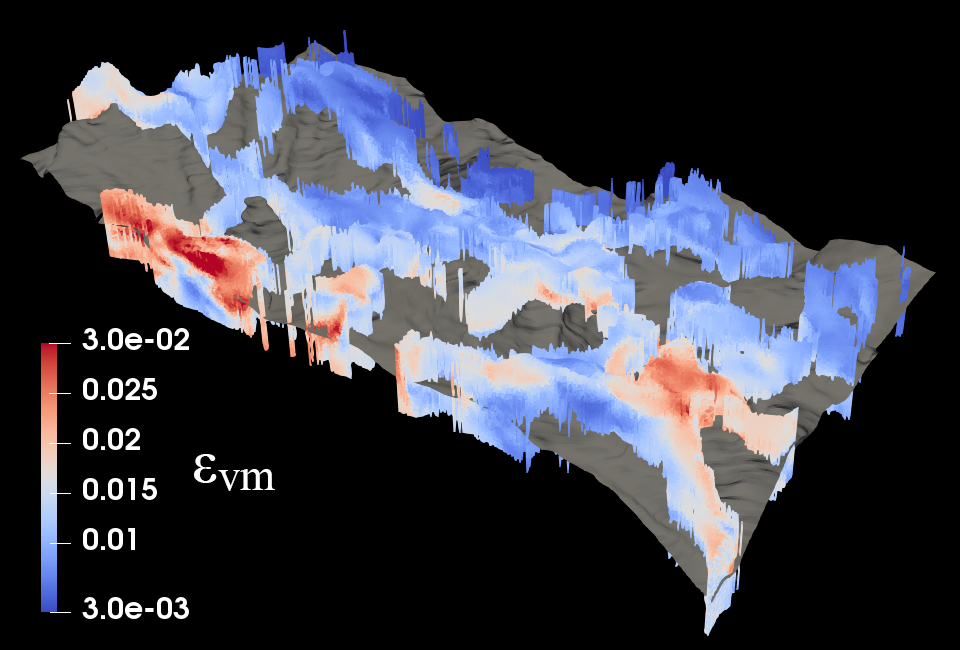
\includegraphics[width=0.5\hsize]{epsilon_vm_regions}
    \caption{Colored data points within $L$ vertical distance of the crack surface that meet the spatial-gradient threshold for inclusion in the correlation analysis of $\epsilon_{vm}$.}
    \label{fig:epsilon_vm_regions}
\end{figure}

This method can be easily parallelized, as computations are performed on each point of the crack surface independently of all other points. Since computations must be performed for each of the $88 \times 383 \times 750 \times 50 = 1.264\times 10^{9}$ points, this parallelization is a necessity.  The data are loaded into shared memory accessible by all processes, after which the code is run on multiple cores. The entire algorithm is described in Fig.~\ref{fig:algorithm}.
\begin{figure}[b]
  \centering
    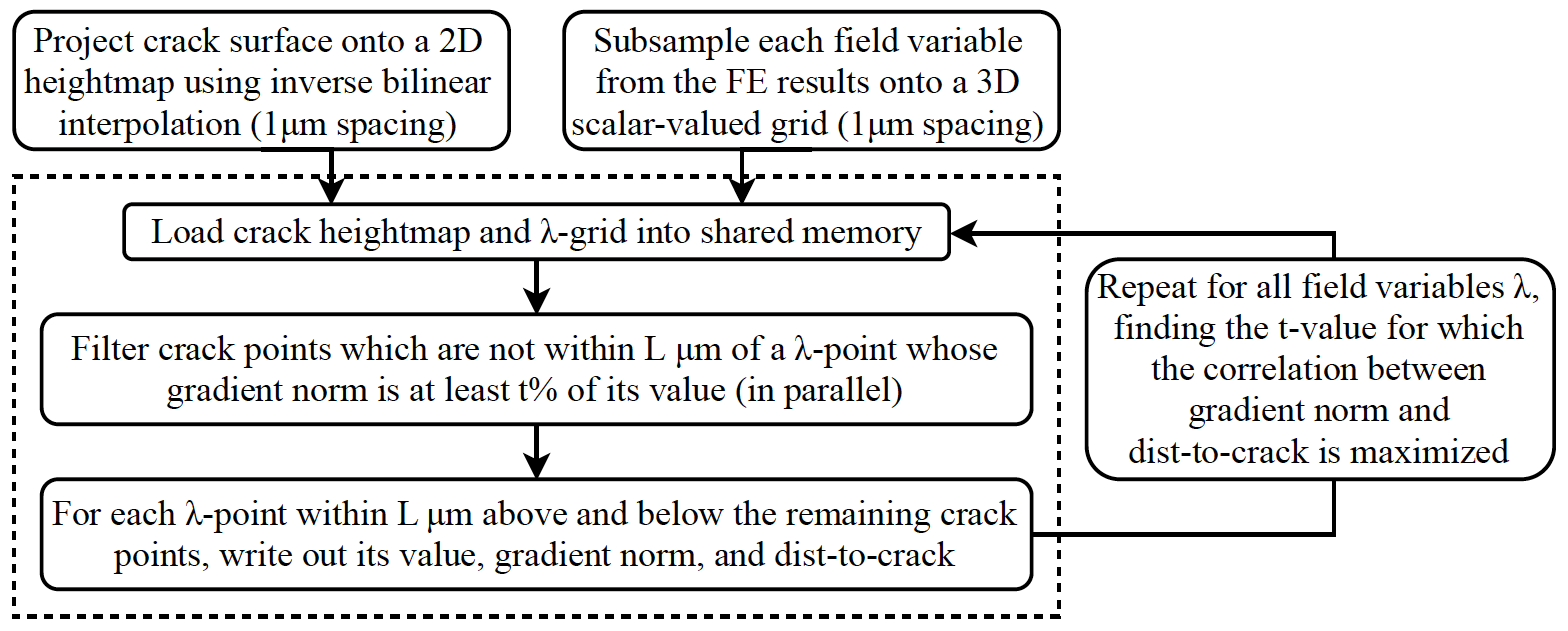
\includegraphics[width=0.75\hsize]{algorithm}
    \caption{Data-extraction algorithm.}
    \label{fig:algorithm}
\end{figure}

The results from the algorithm consist of data frames, where each row is an observed point from the microstructure and each column is the value of a field variable, or distance to crack surface in the case of the last column. These data frames are then imported into R \cite{statistical2009r}, which provides robust libraries for correlation analyses and visualizations. Pearson correlation coefficients are computed for each column with respect to the final column, and then visualized for comparison.

\section{Results and discussion}\label{results}
The computed fields for all 22 metrics and their respective cyclic values are visualized for the uncracked microstructure in Figs.~\ref{fig:epsilons}, ~\ref{fig:depsilons}, ~\ref{fig:epsilon_other}, ~\ref{fig:sigmas}, ~\ref{fig:dsigmas}, ~\ref{fig:sigma_other}, ~\ref{fig:Ds}, and ~\ref{fig:dDs}. The computed correlation coefficients are shown in Fig.~\ref{fig:correlations}. A negative correlation indicates that as the distance to crack surface decreases, the variable of interest increases, and vice versa.

\begin{figure}[p]
  \centering
    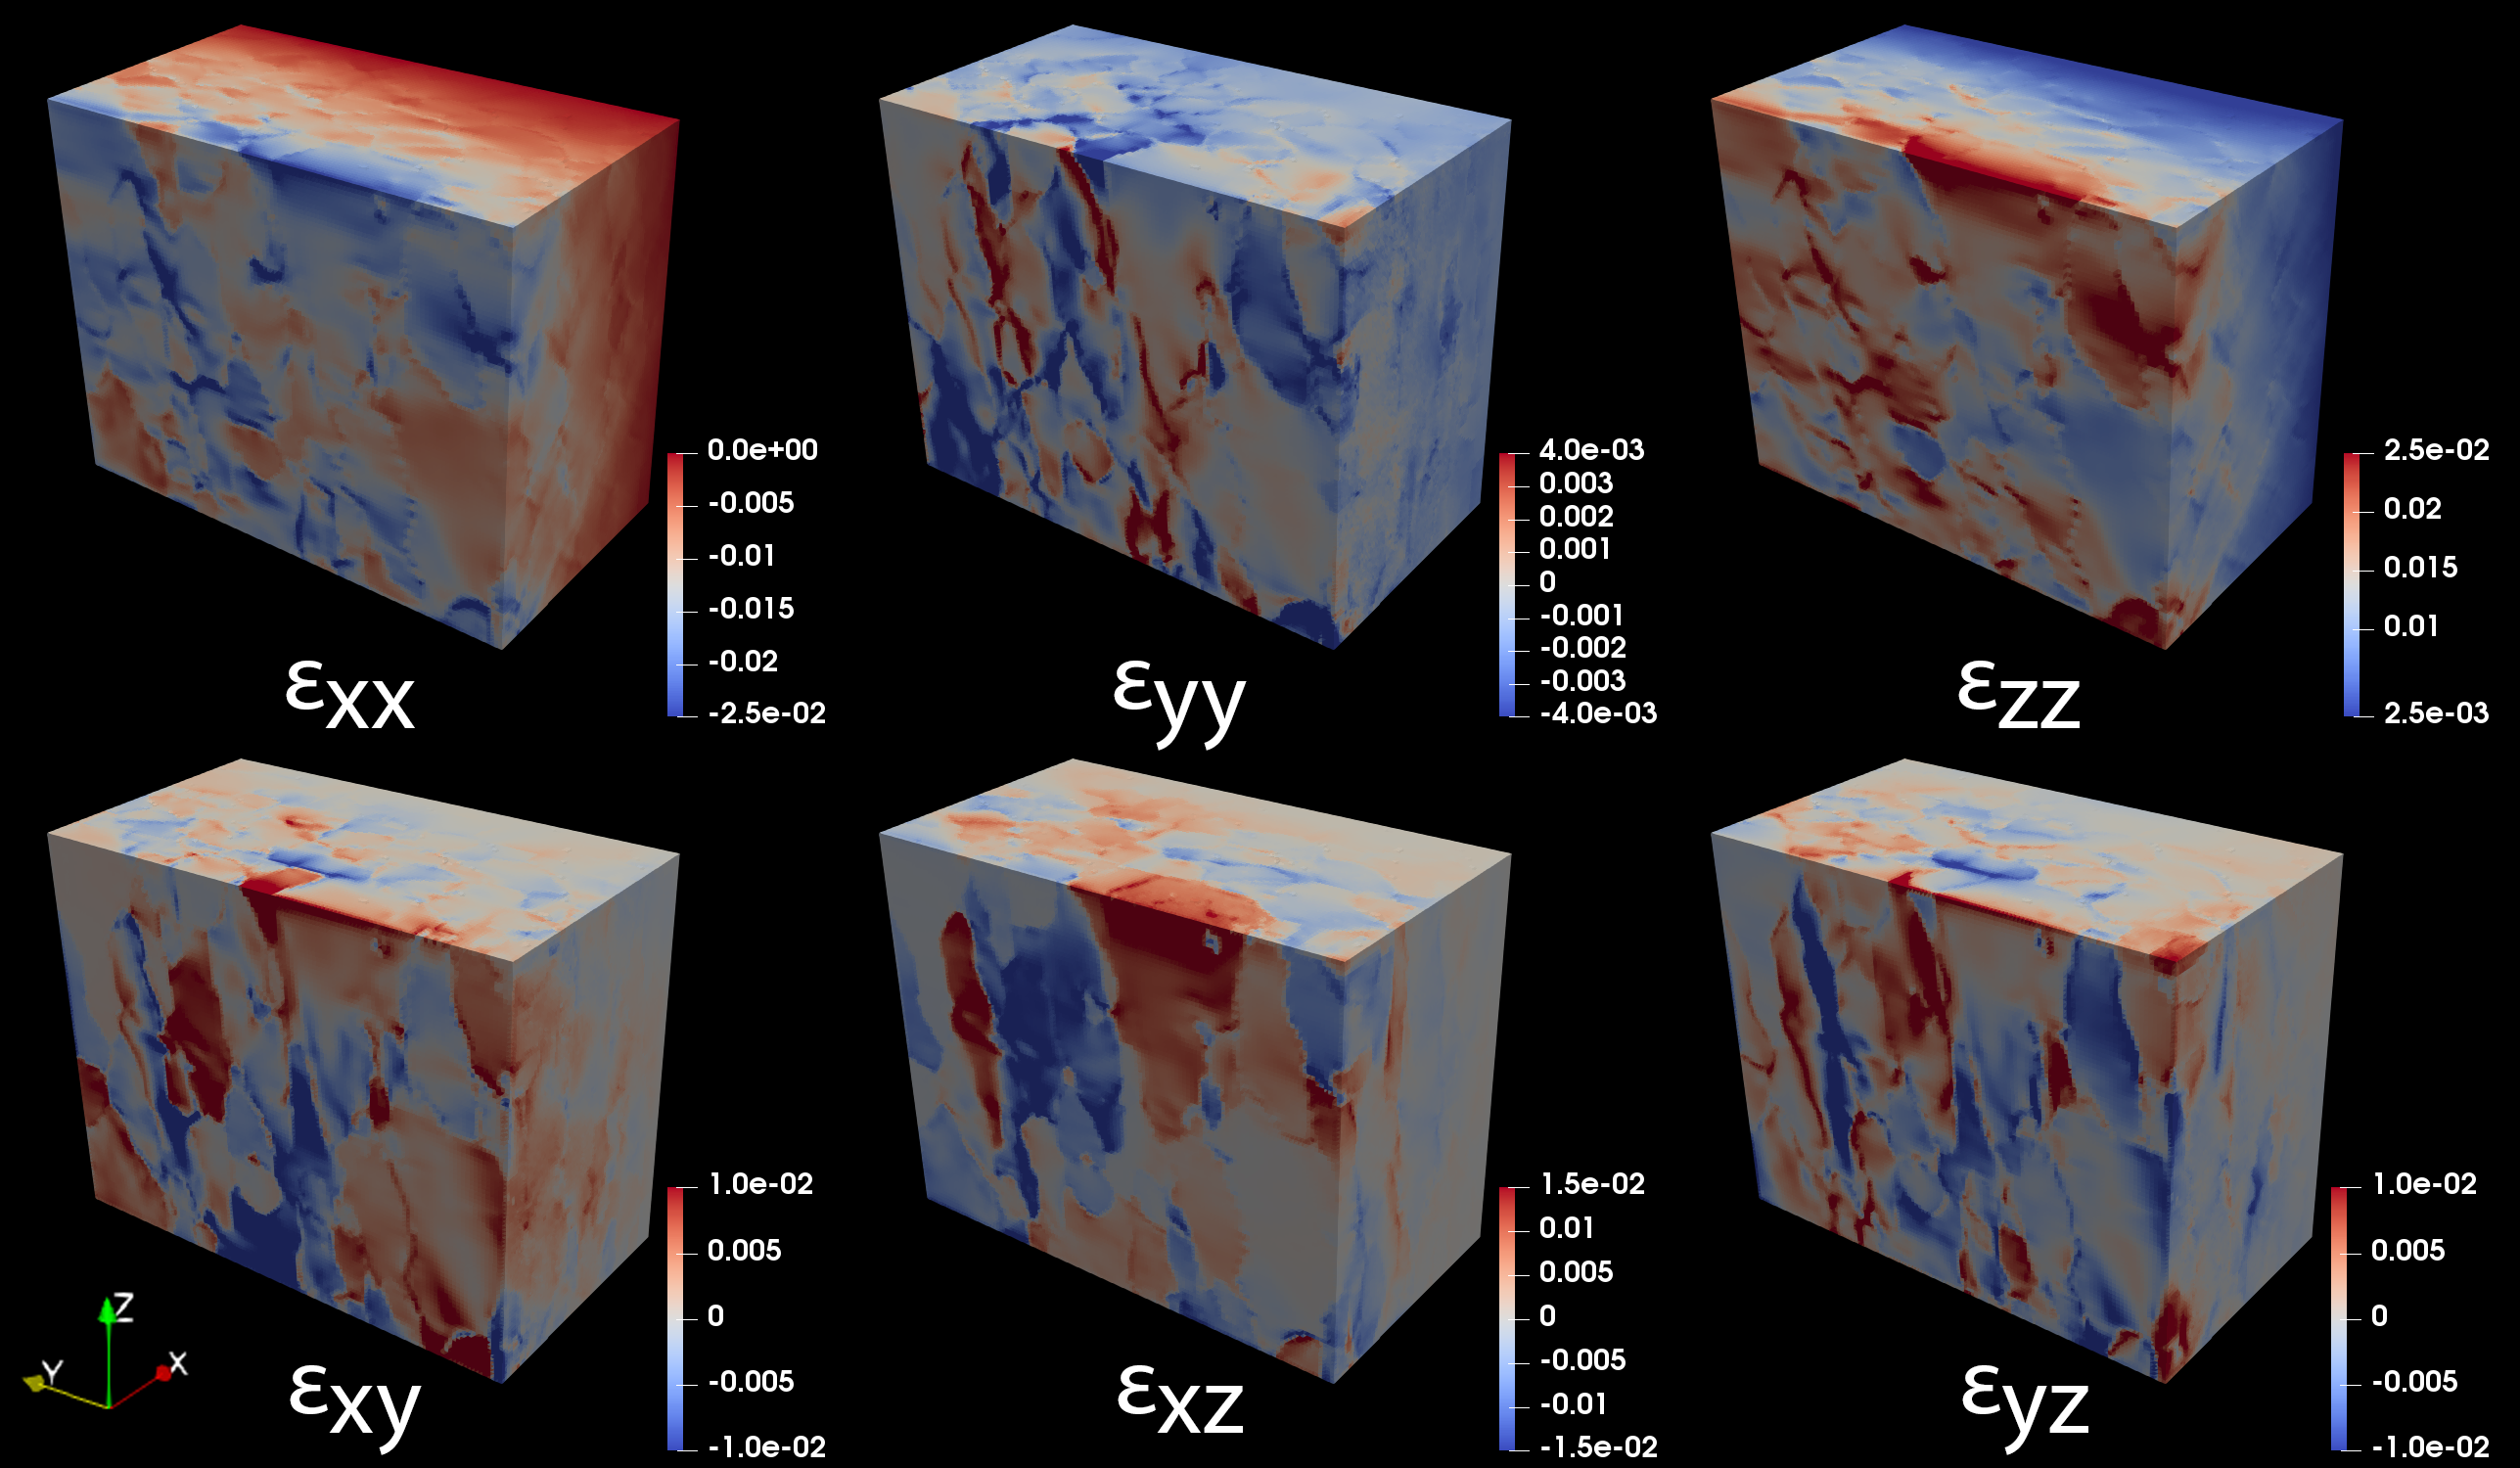
\includegraphics[width=\hsize]{epsilons}
    \captionof{figure}{Grid data showing strain-tensor components computed at the peak load of the fifth loading cycle for an uncracked microstructure in a multi-scale finite-element simulation.}
    \label{fig:epsilons}
\end{figure}

\begin{figure}[p]
  \centering
    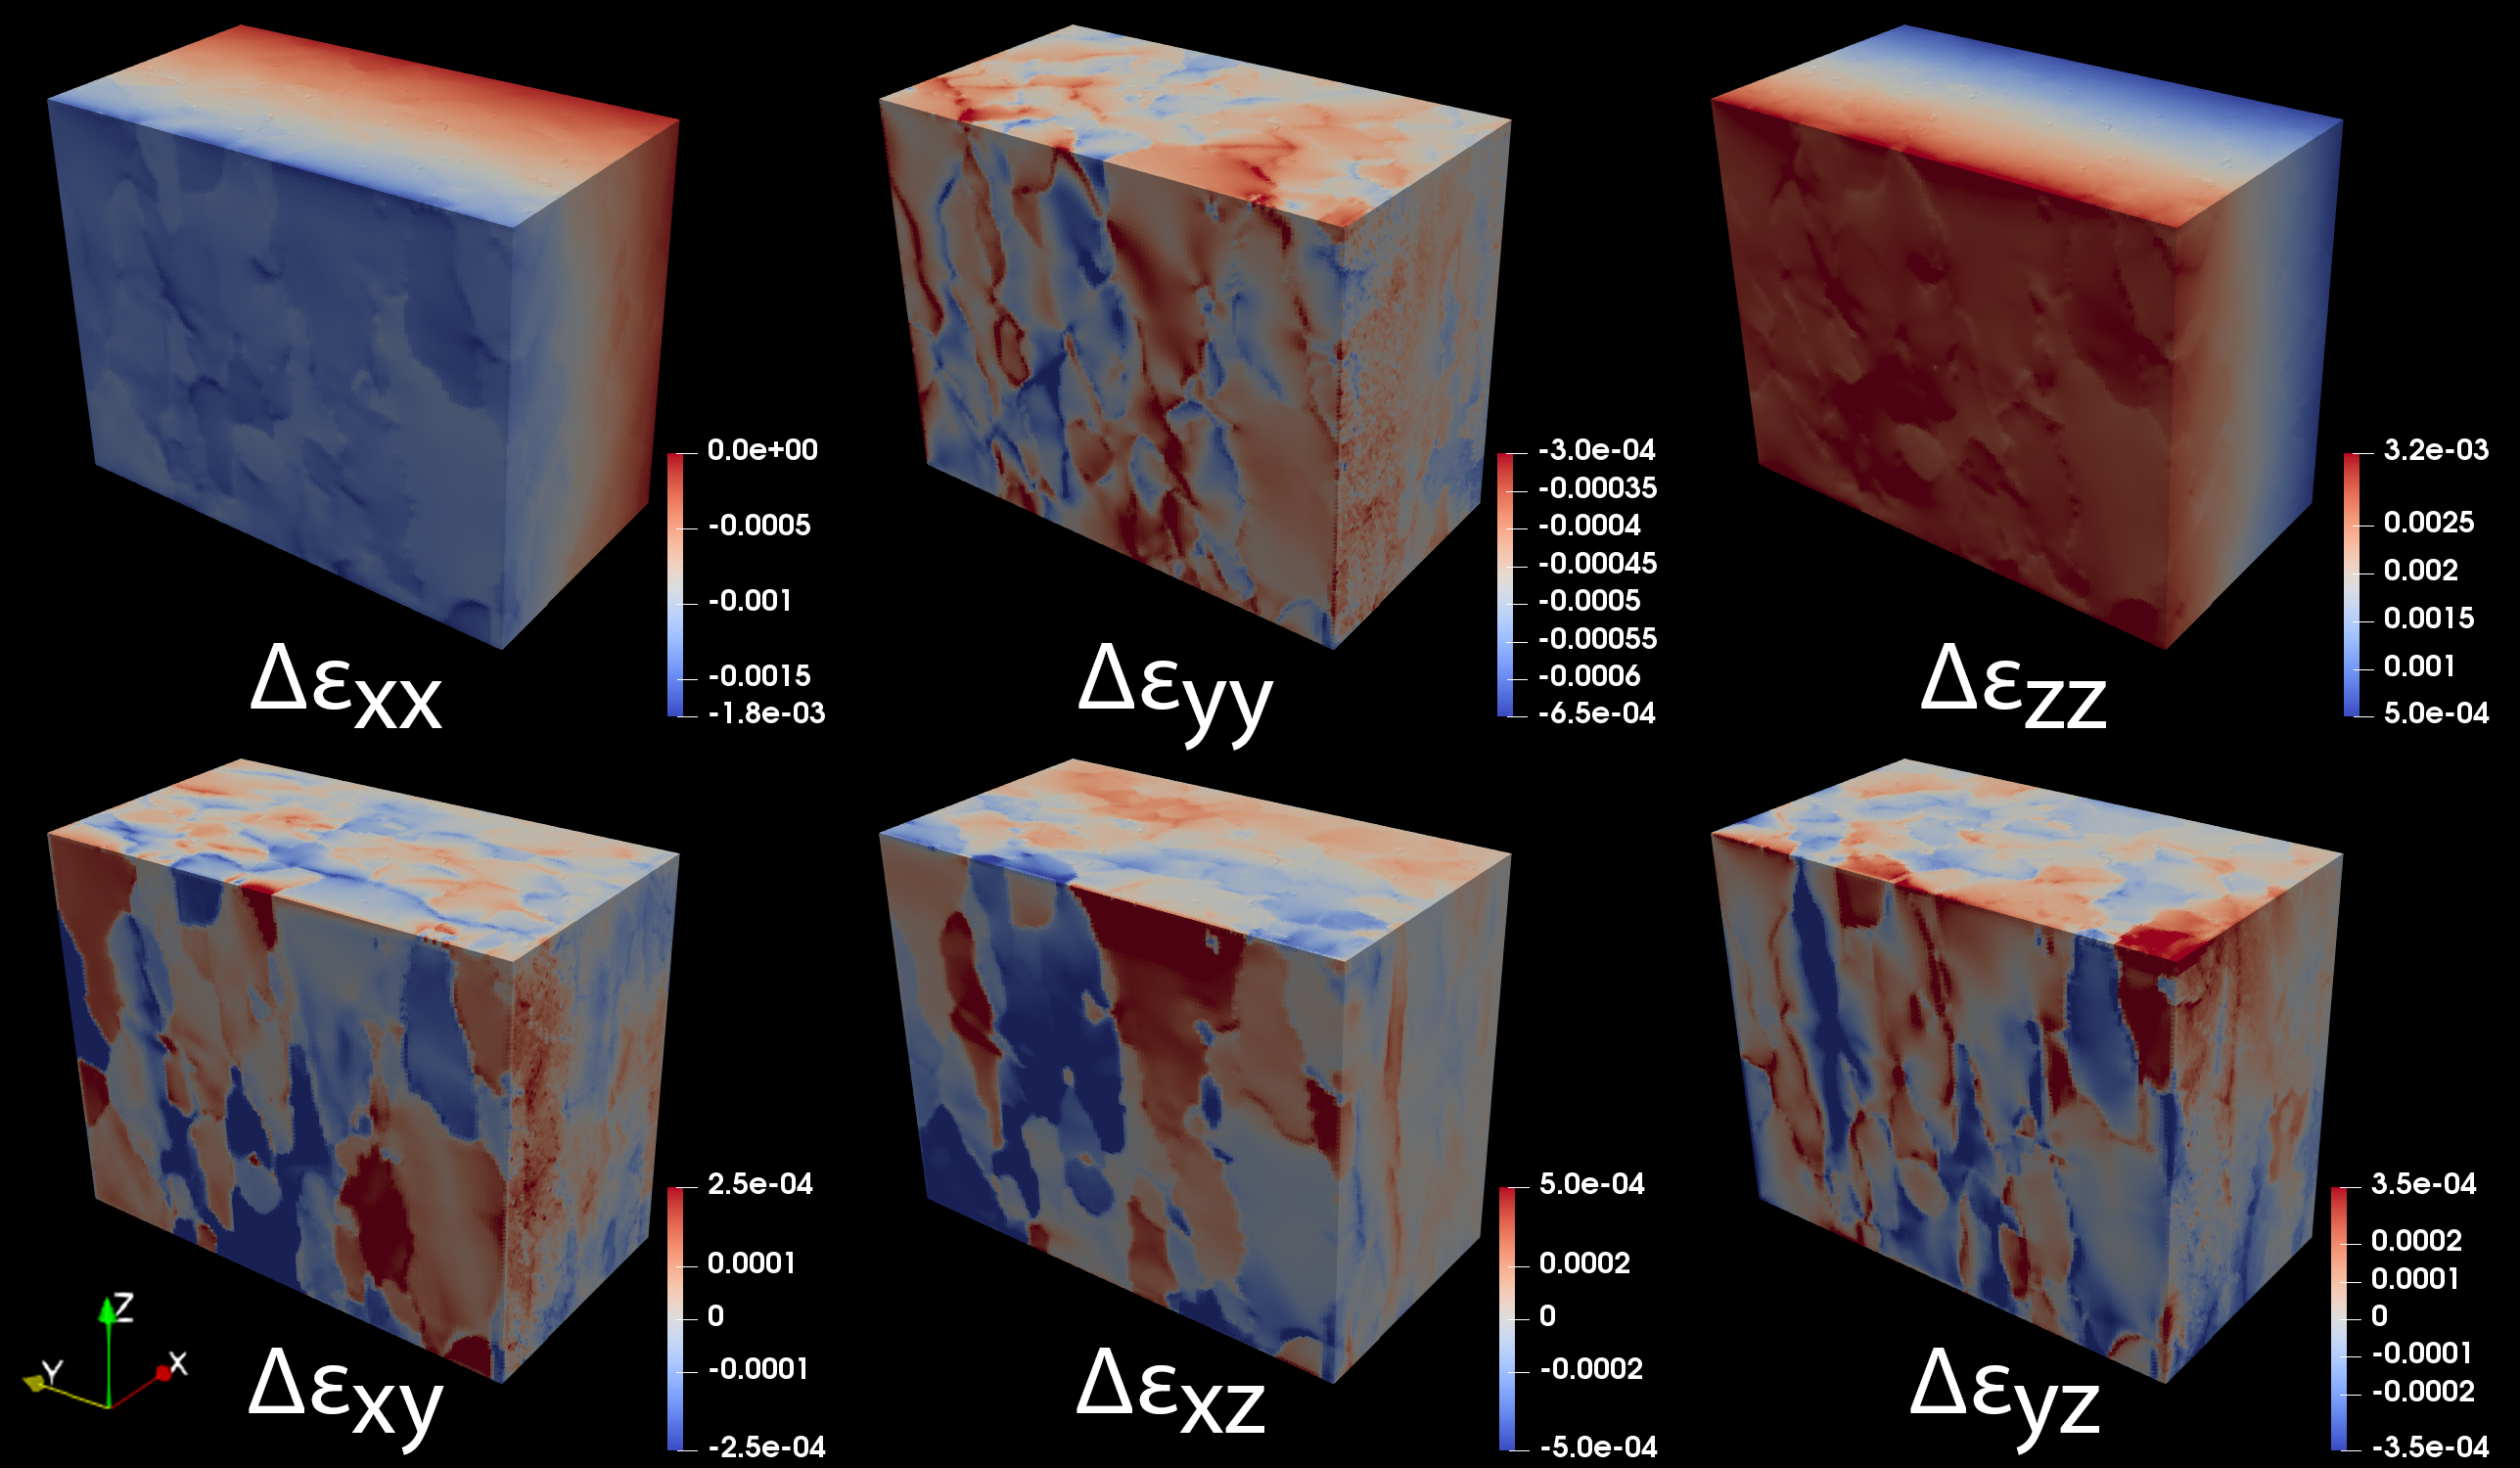
\includegraphics[width=\hsize]{depsilons}
    \caption{Grid data showing cyclic values of the strain-tensor components computed for an uncracked microstructure in a multi-scale finite-element simulation.}
    \label{fig:depsilons}
\end{figure}

\begin{figure}[p]
  \centering
    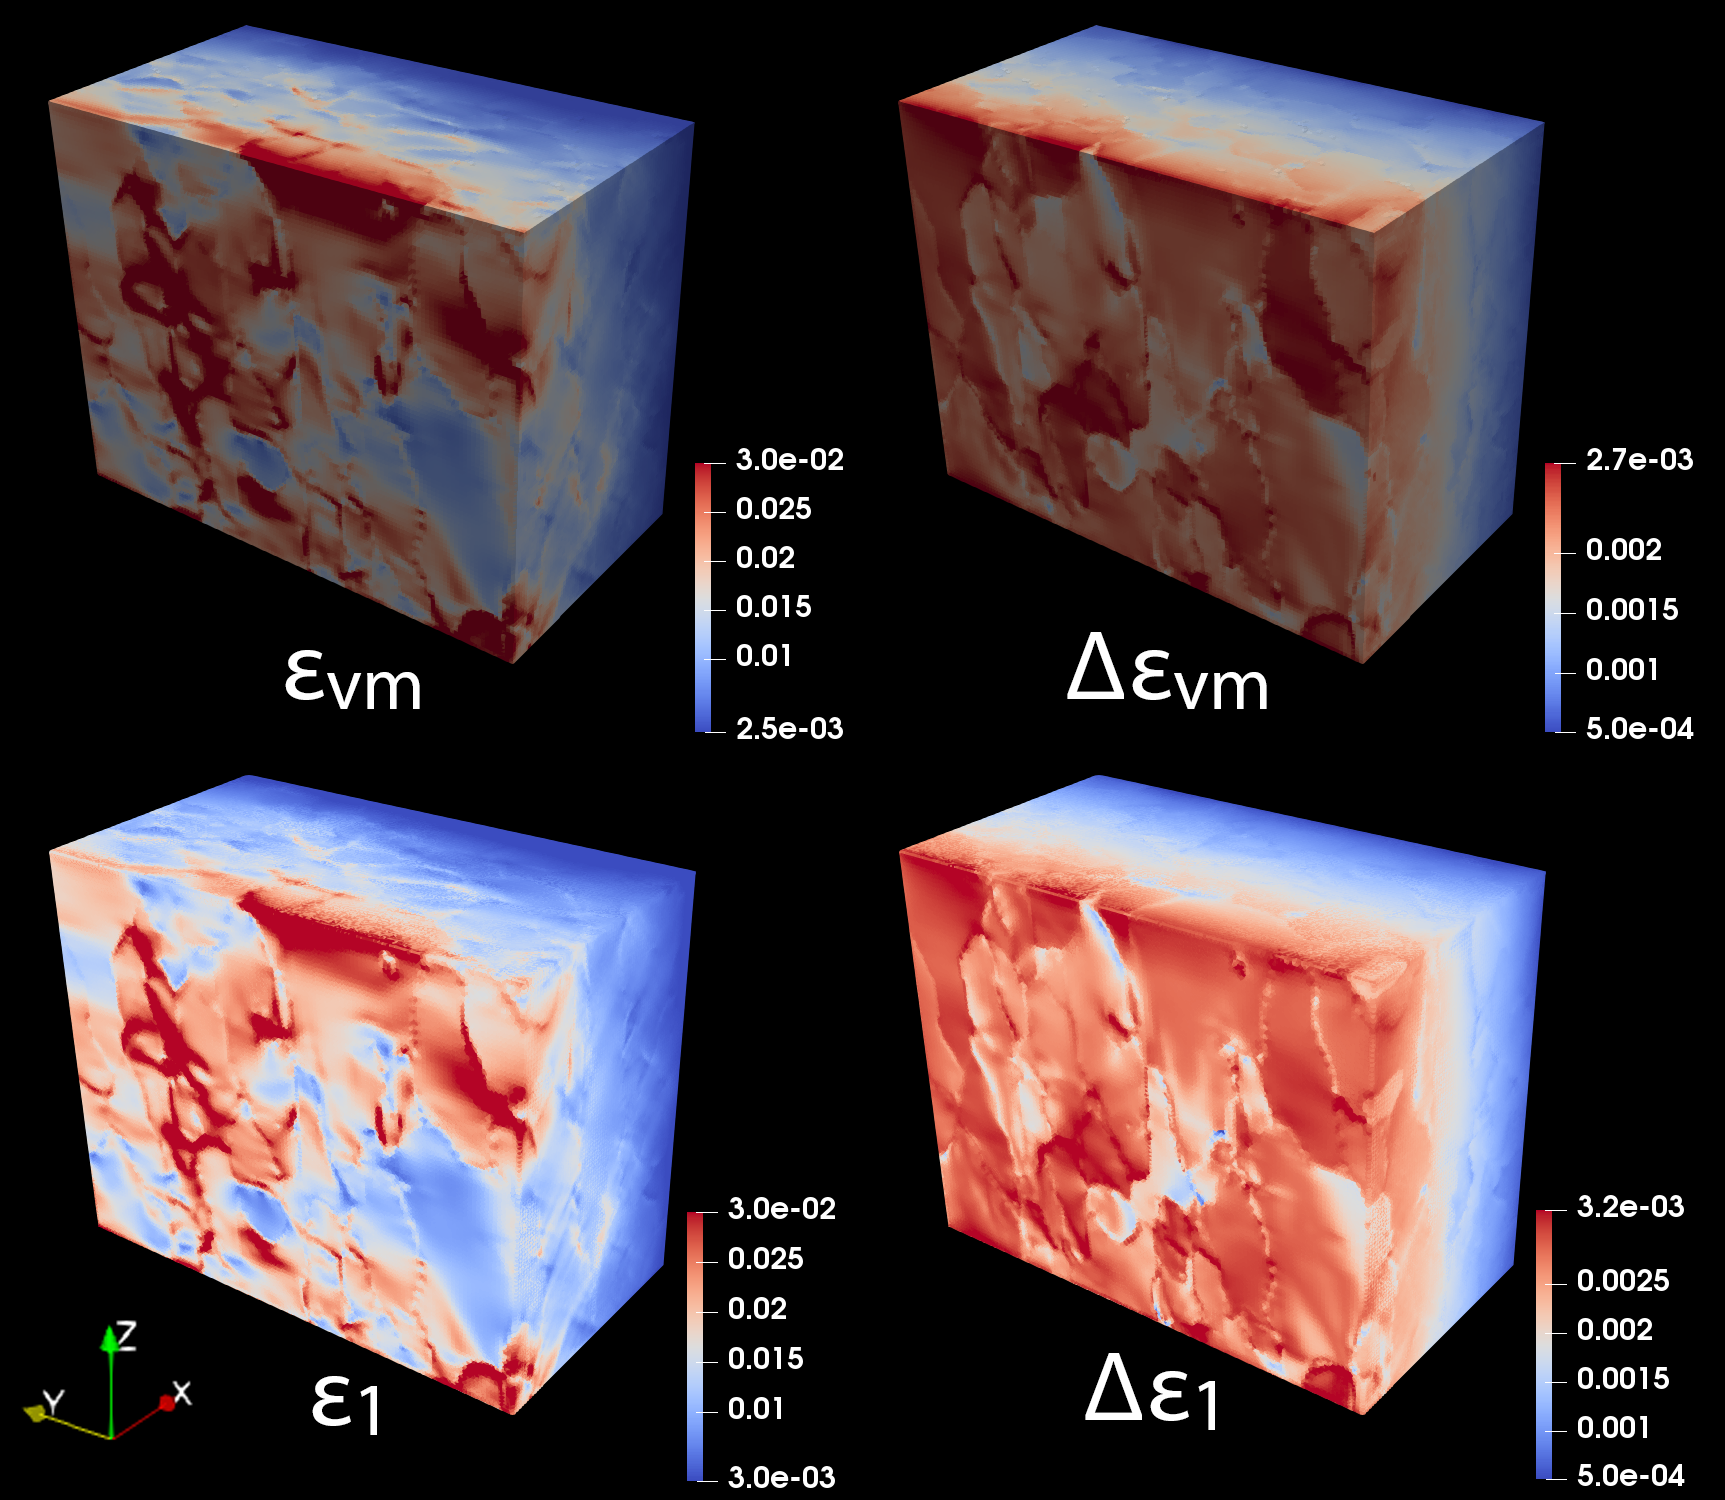
\includegraphics[width=\hsize]{epsilon_other}
    \caption{Grid data showing von-Mises and maximum-principal strains computed at the peak load of the fifth loading cycle (left) and the corresponding cyclic values (right) for an uncracked microstructure in a multi-scale finite-element simulation.}
    \label{fig:epsilon_other}
\end{figure}

\begin{figure}[p]
  \centering
    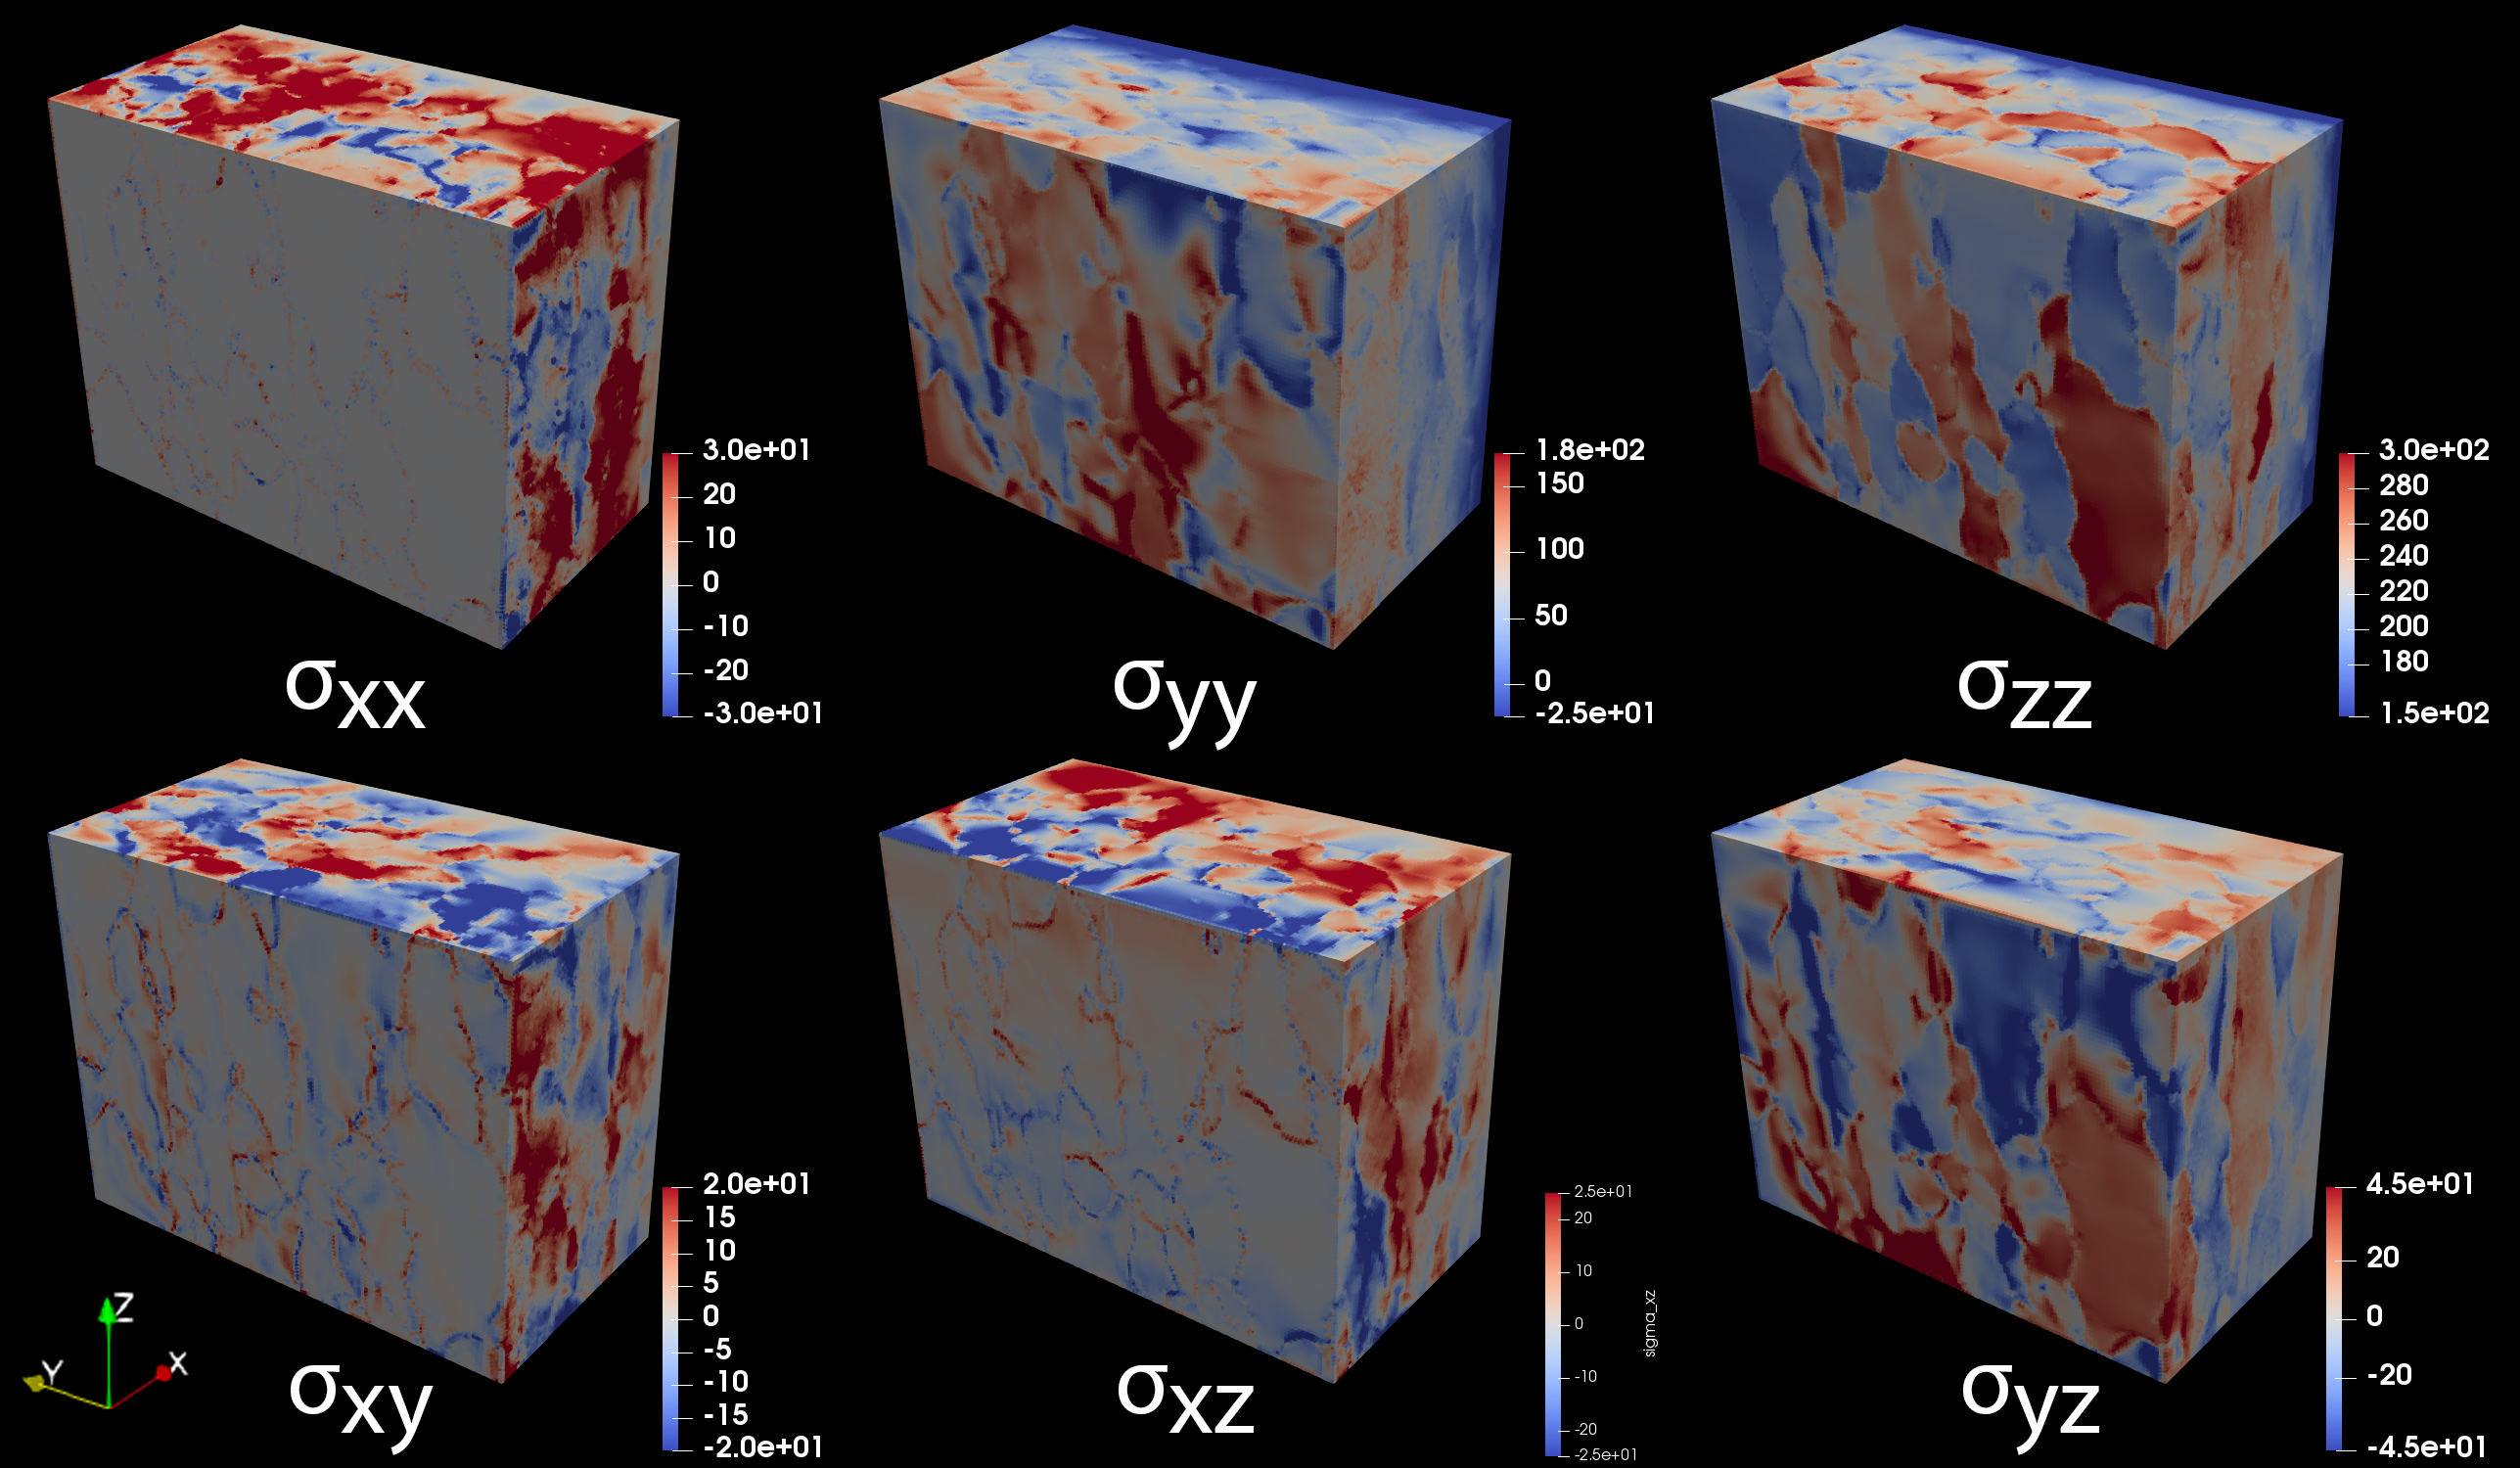
\includegraphics[width=\hsize]{sigmas}
    \caption{Grid data showing stress-tensor components (MPa) computed at the peak load of the fifth loading cycle for an uncracked microstructure in a multi-scale finite-element simulation.}
    \label{fig:sigmas}
\end{figure}

\begin{figure}[p]
  \centering
    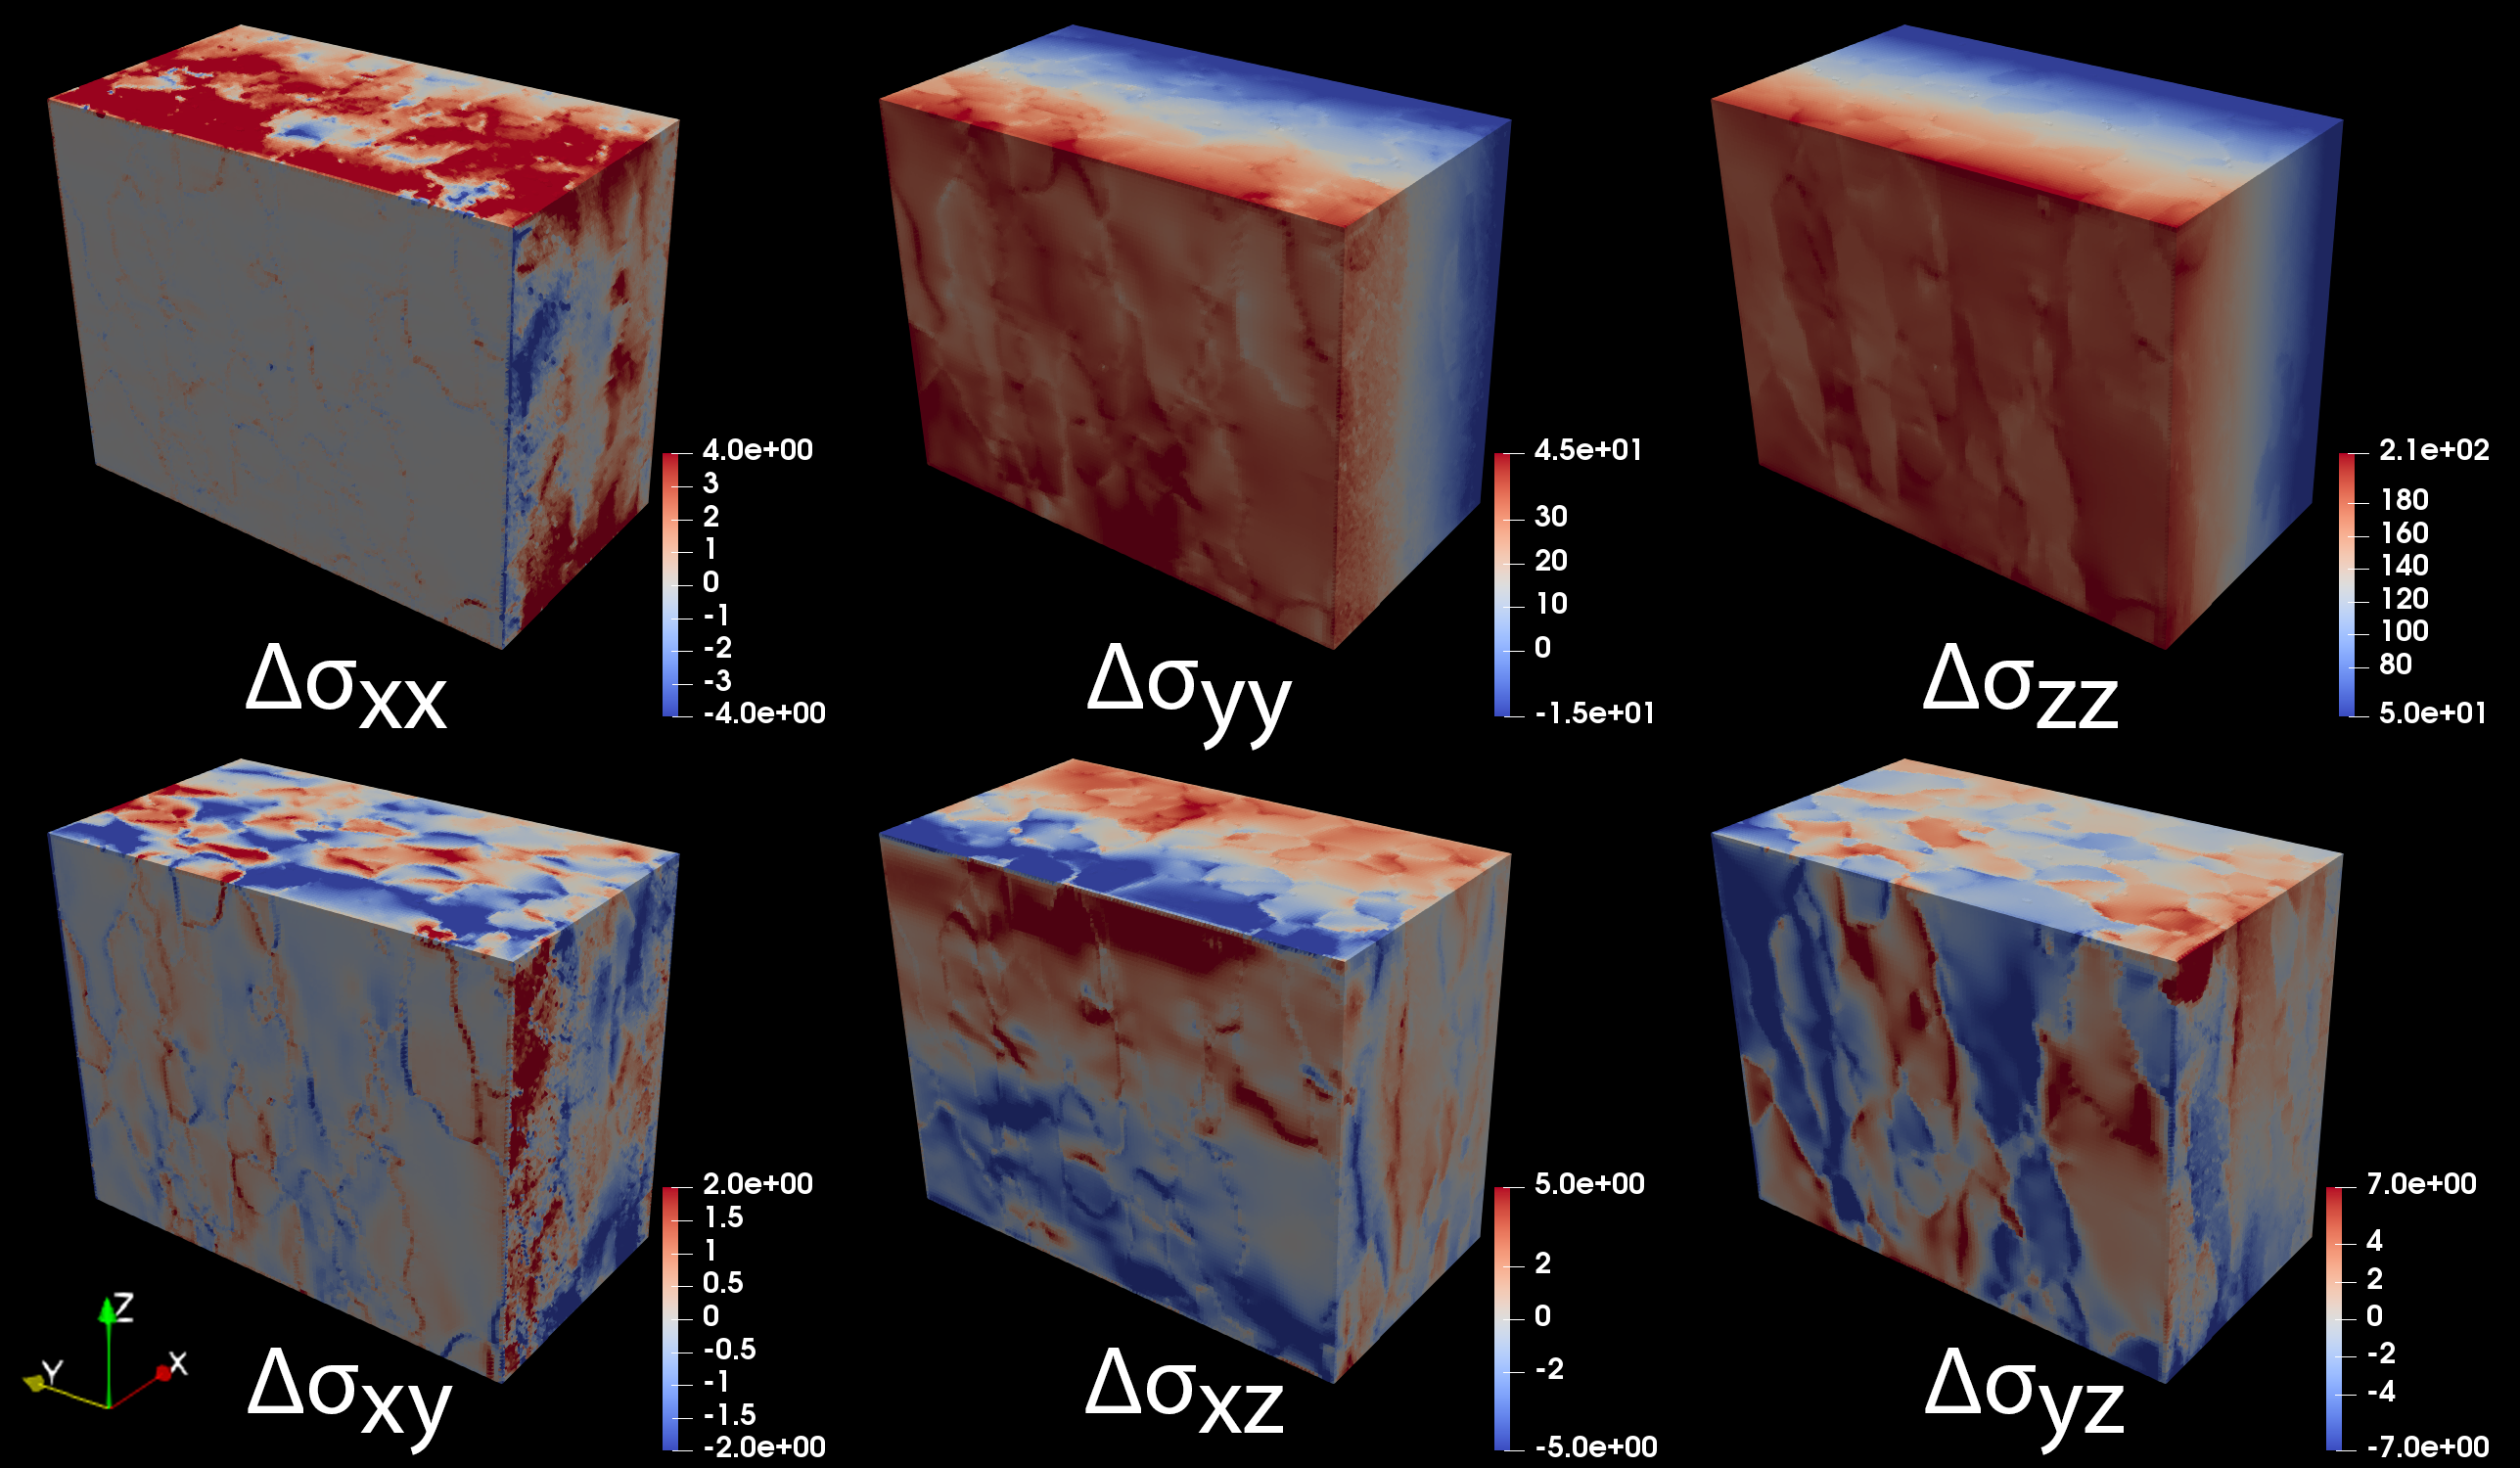
\includegraphics[width=\hsize]{dsigmas}
    \caption{Grid data showing cyclic values of the stress-tensor components (MPa) computed for an uncracked microstructure in a multi-scale finite-element simulation.}
    \label{fig:dsigmas}
\end{figure}

\begin{figure}[p]
  \centering
    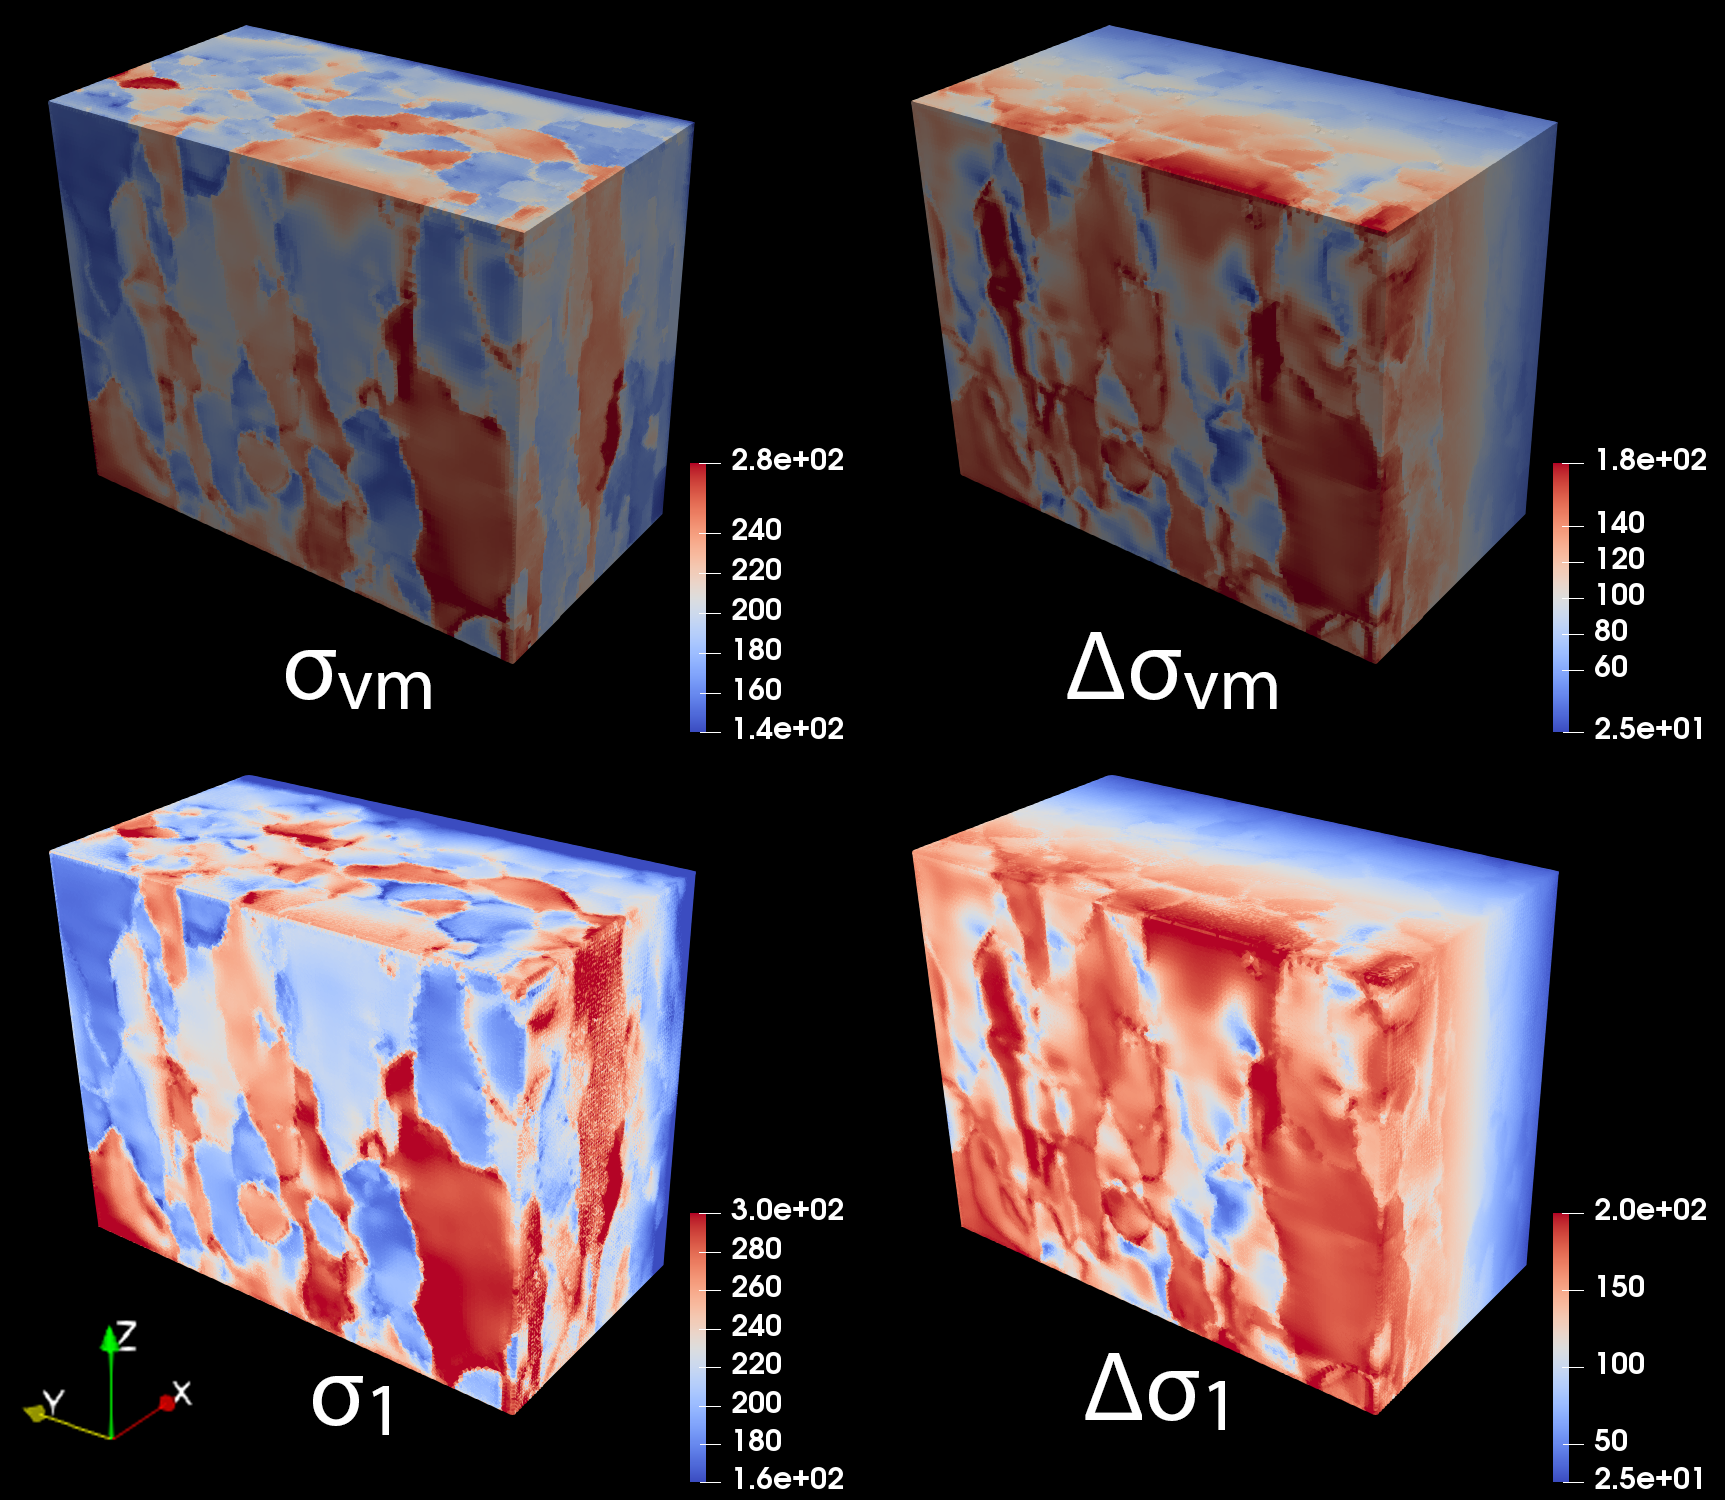
\includegraphics[width=\hsize]{sigma_other}
    \caption{Grid data showing von-Mises and maximum-principal stresses (MPa) computed at the peak load of the fifth loading cycle (left) and the corresponding cyclic values (right) for an uncracked microstructure in a multi-scale finite-element simulation.}
    \label{fig:sigma_other}
\end{figure}

\begin{figure}[p]
  \centering
    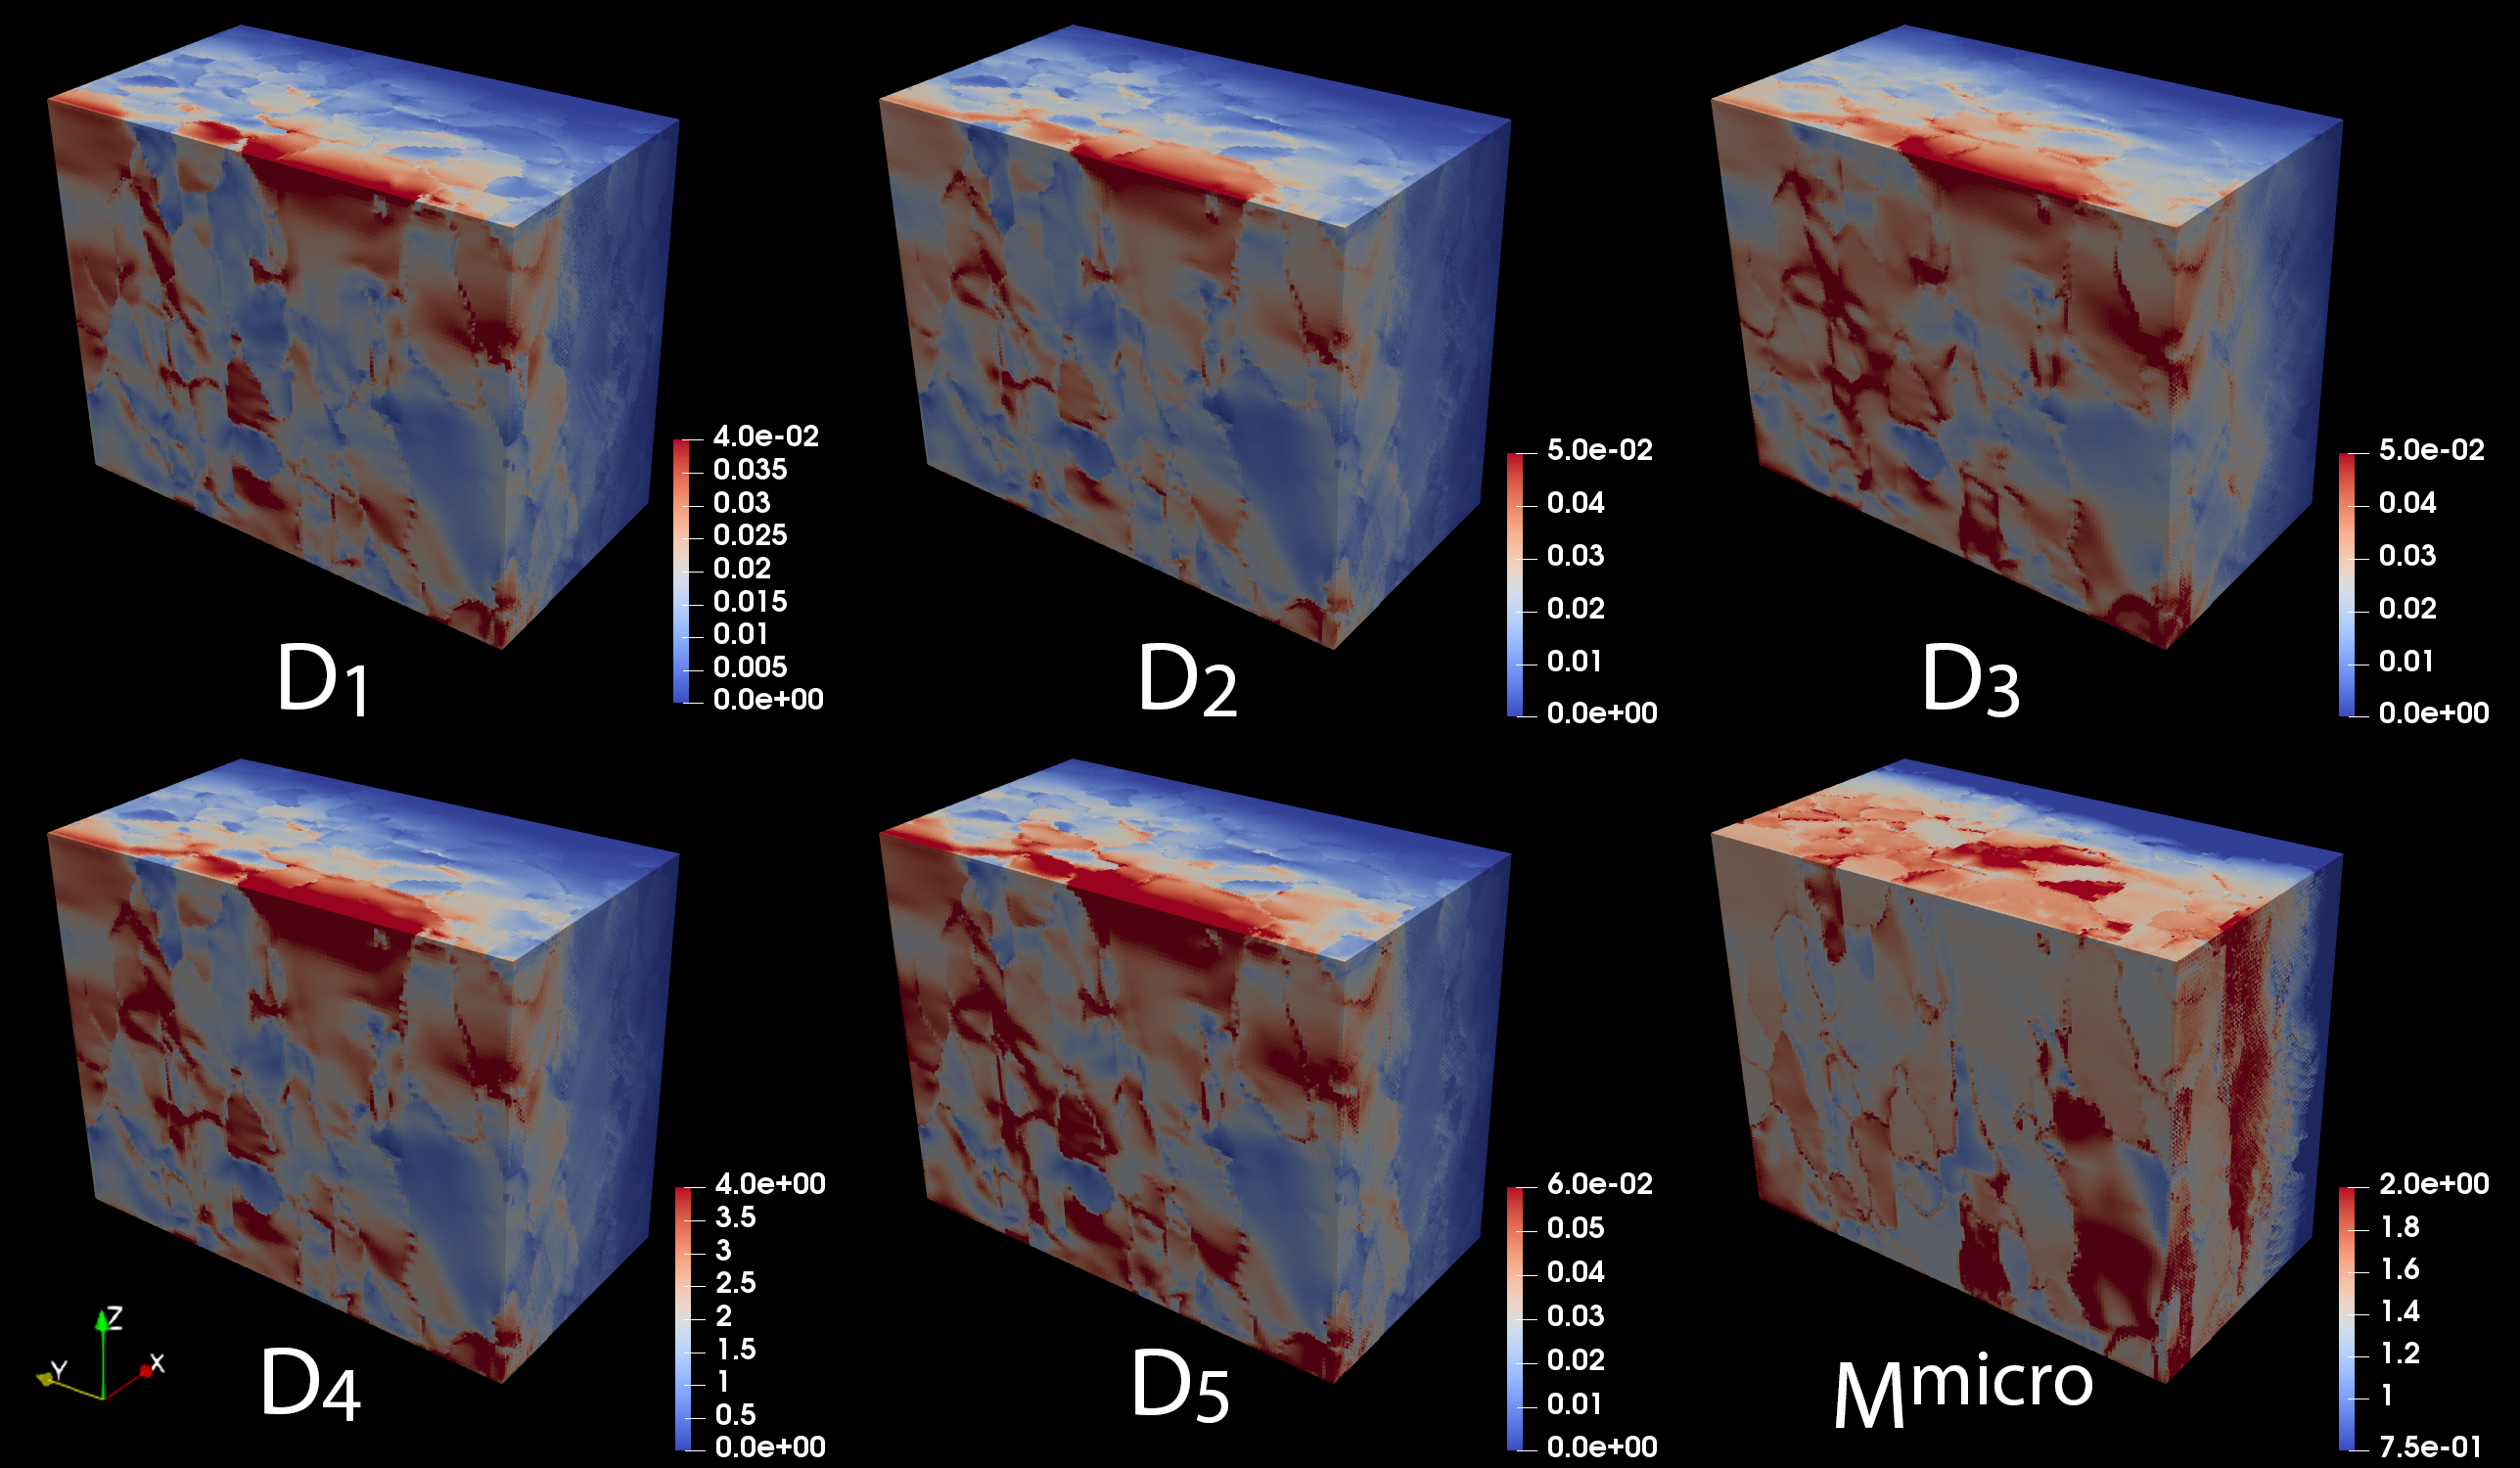
\includegraphics[width=\hsize]{Ds}
    \caption{Grid data showing slip-based damage metrics computed at the peak load of the fifth loading cycle for an uncracked microstructure in a multi-scale finite-element simulation.}
    \label{fig:Ds}
\end{figure}

\begin{figure}[p]
  \centering
    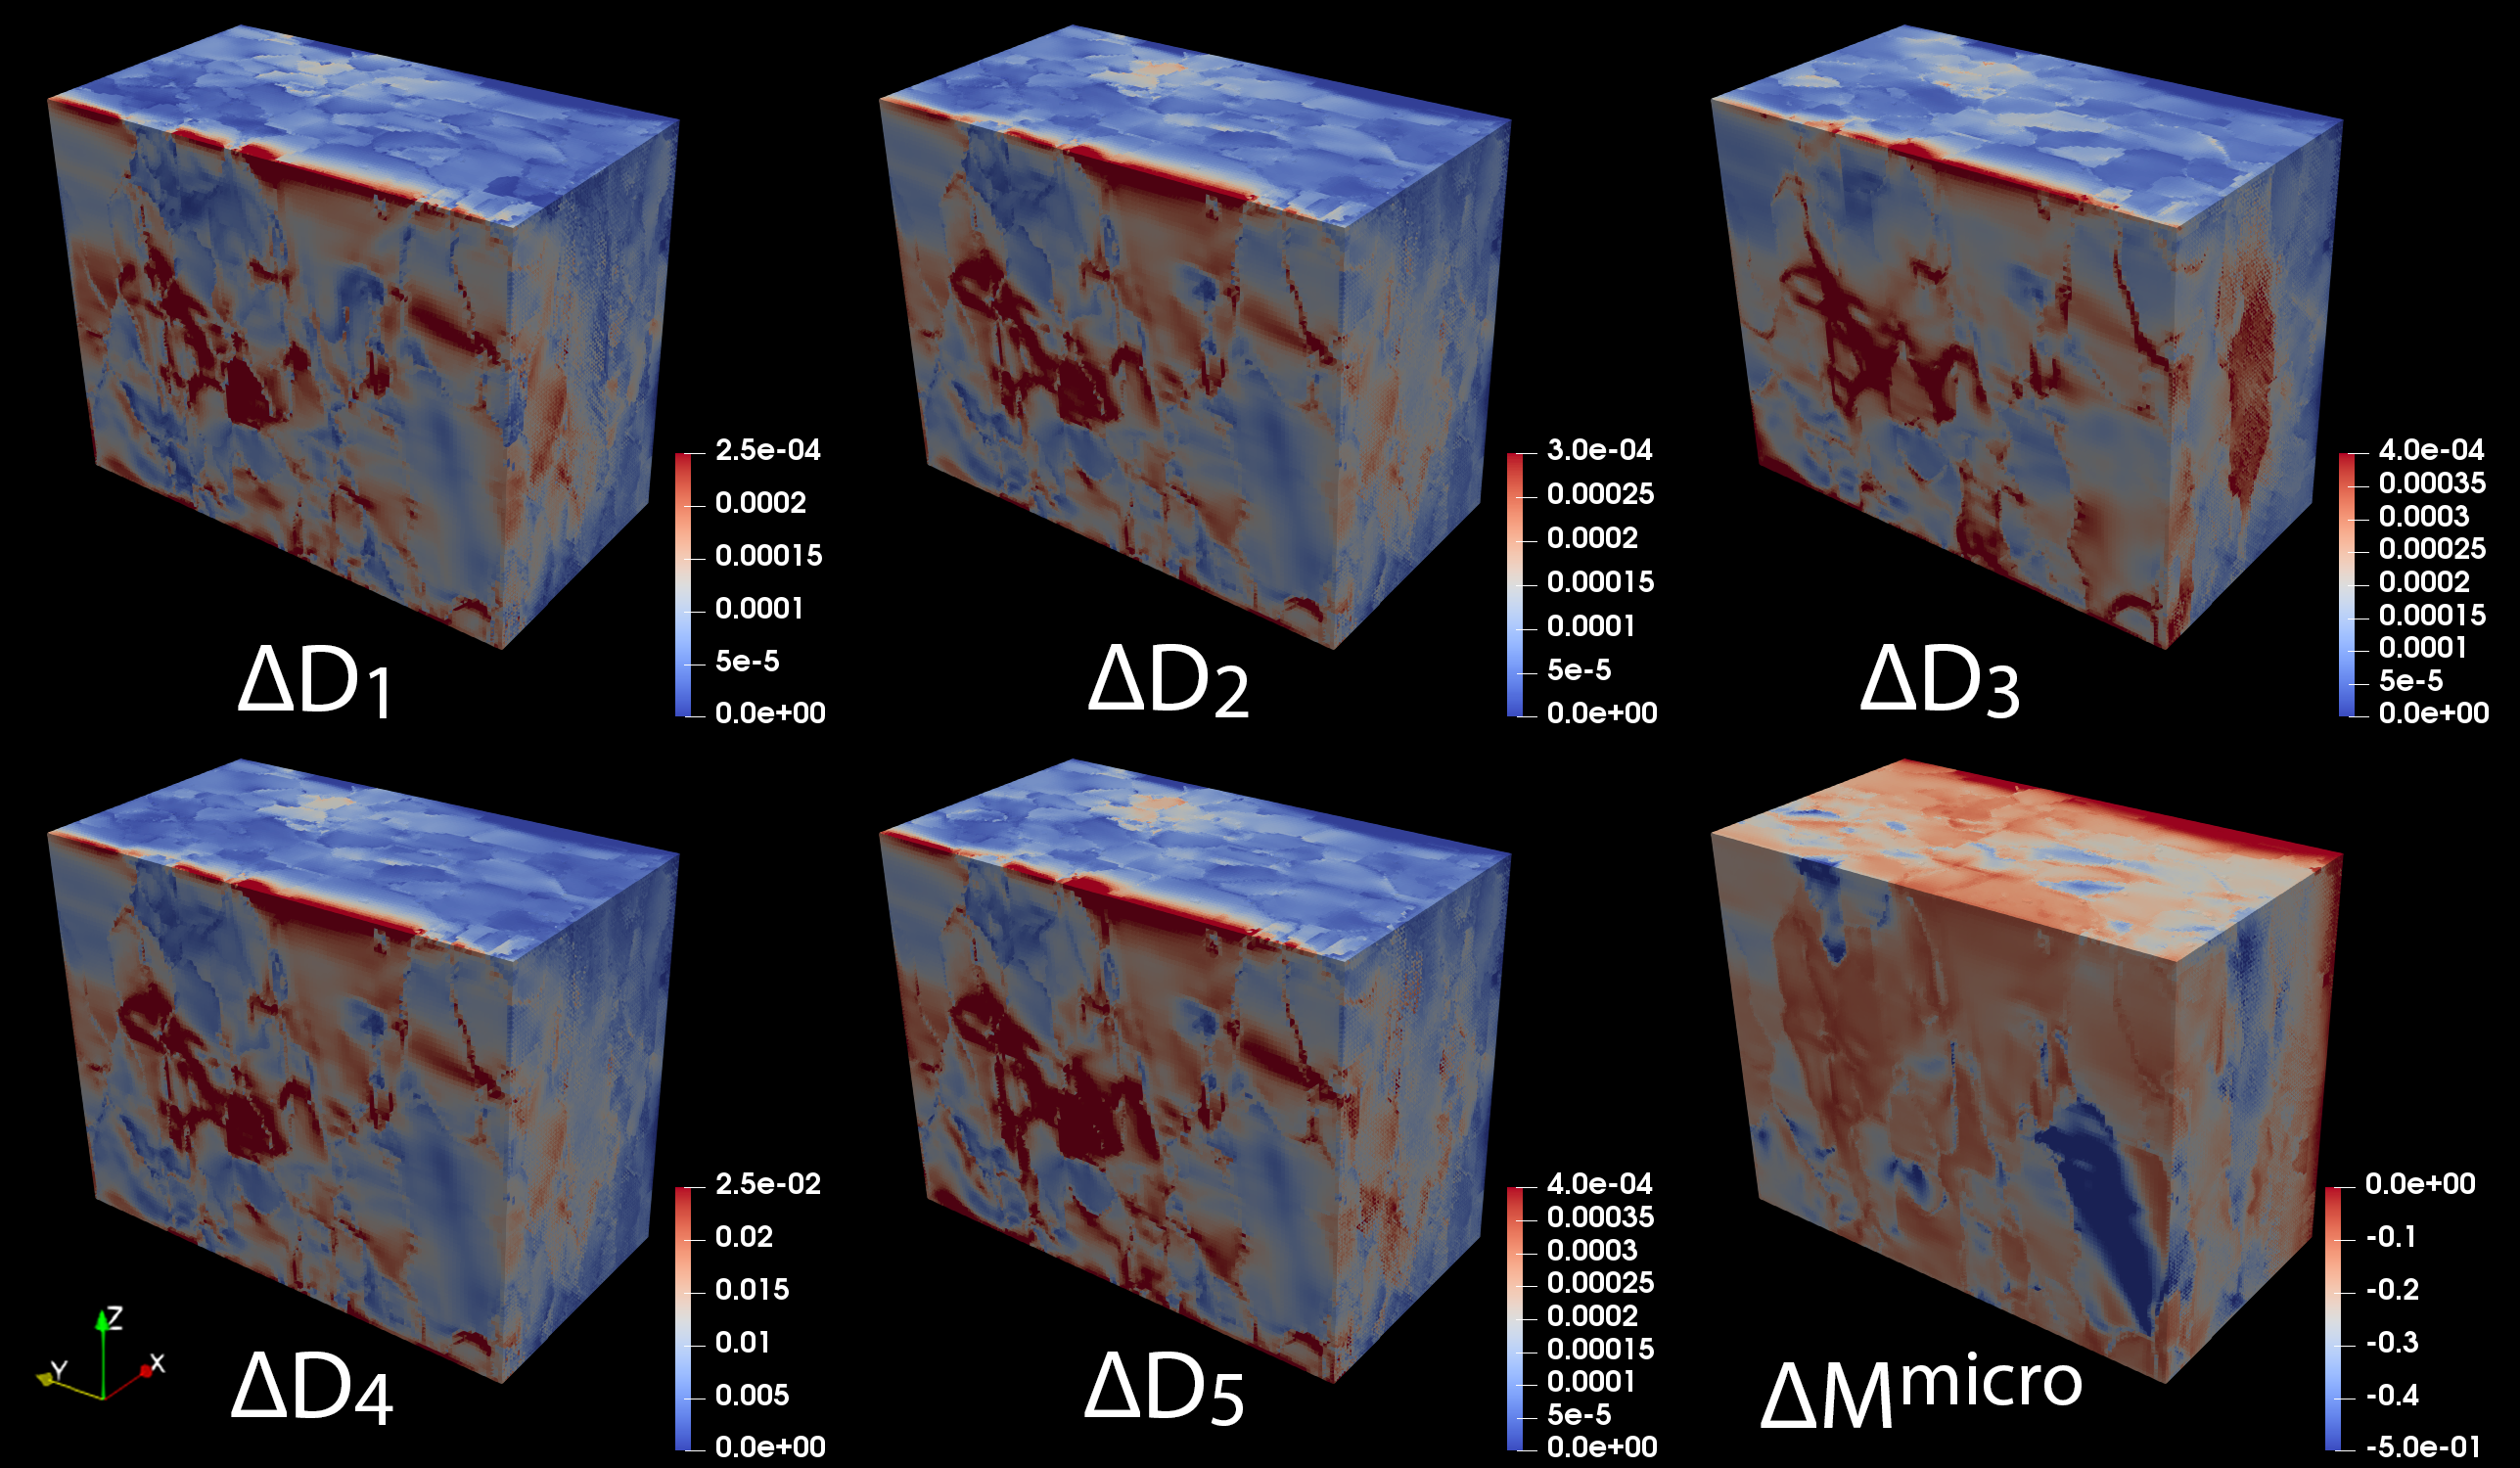
\includegraphics[width=\hsize]{dDs}
    \caption{Grid data showing cyclic values of the slip-based damage metrics computed for an uncracked microstructure in a multi-scale finite-element simulation.}
    \label{fig:dDs}
\end{figure}

\begin{figure}[p]
  \centering
    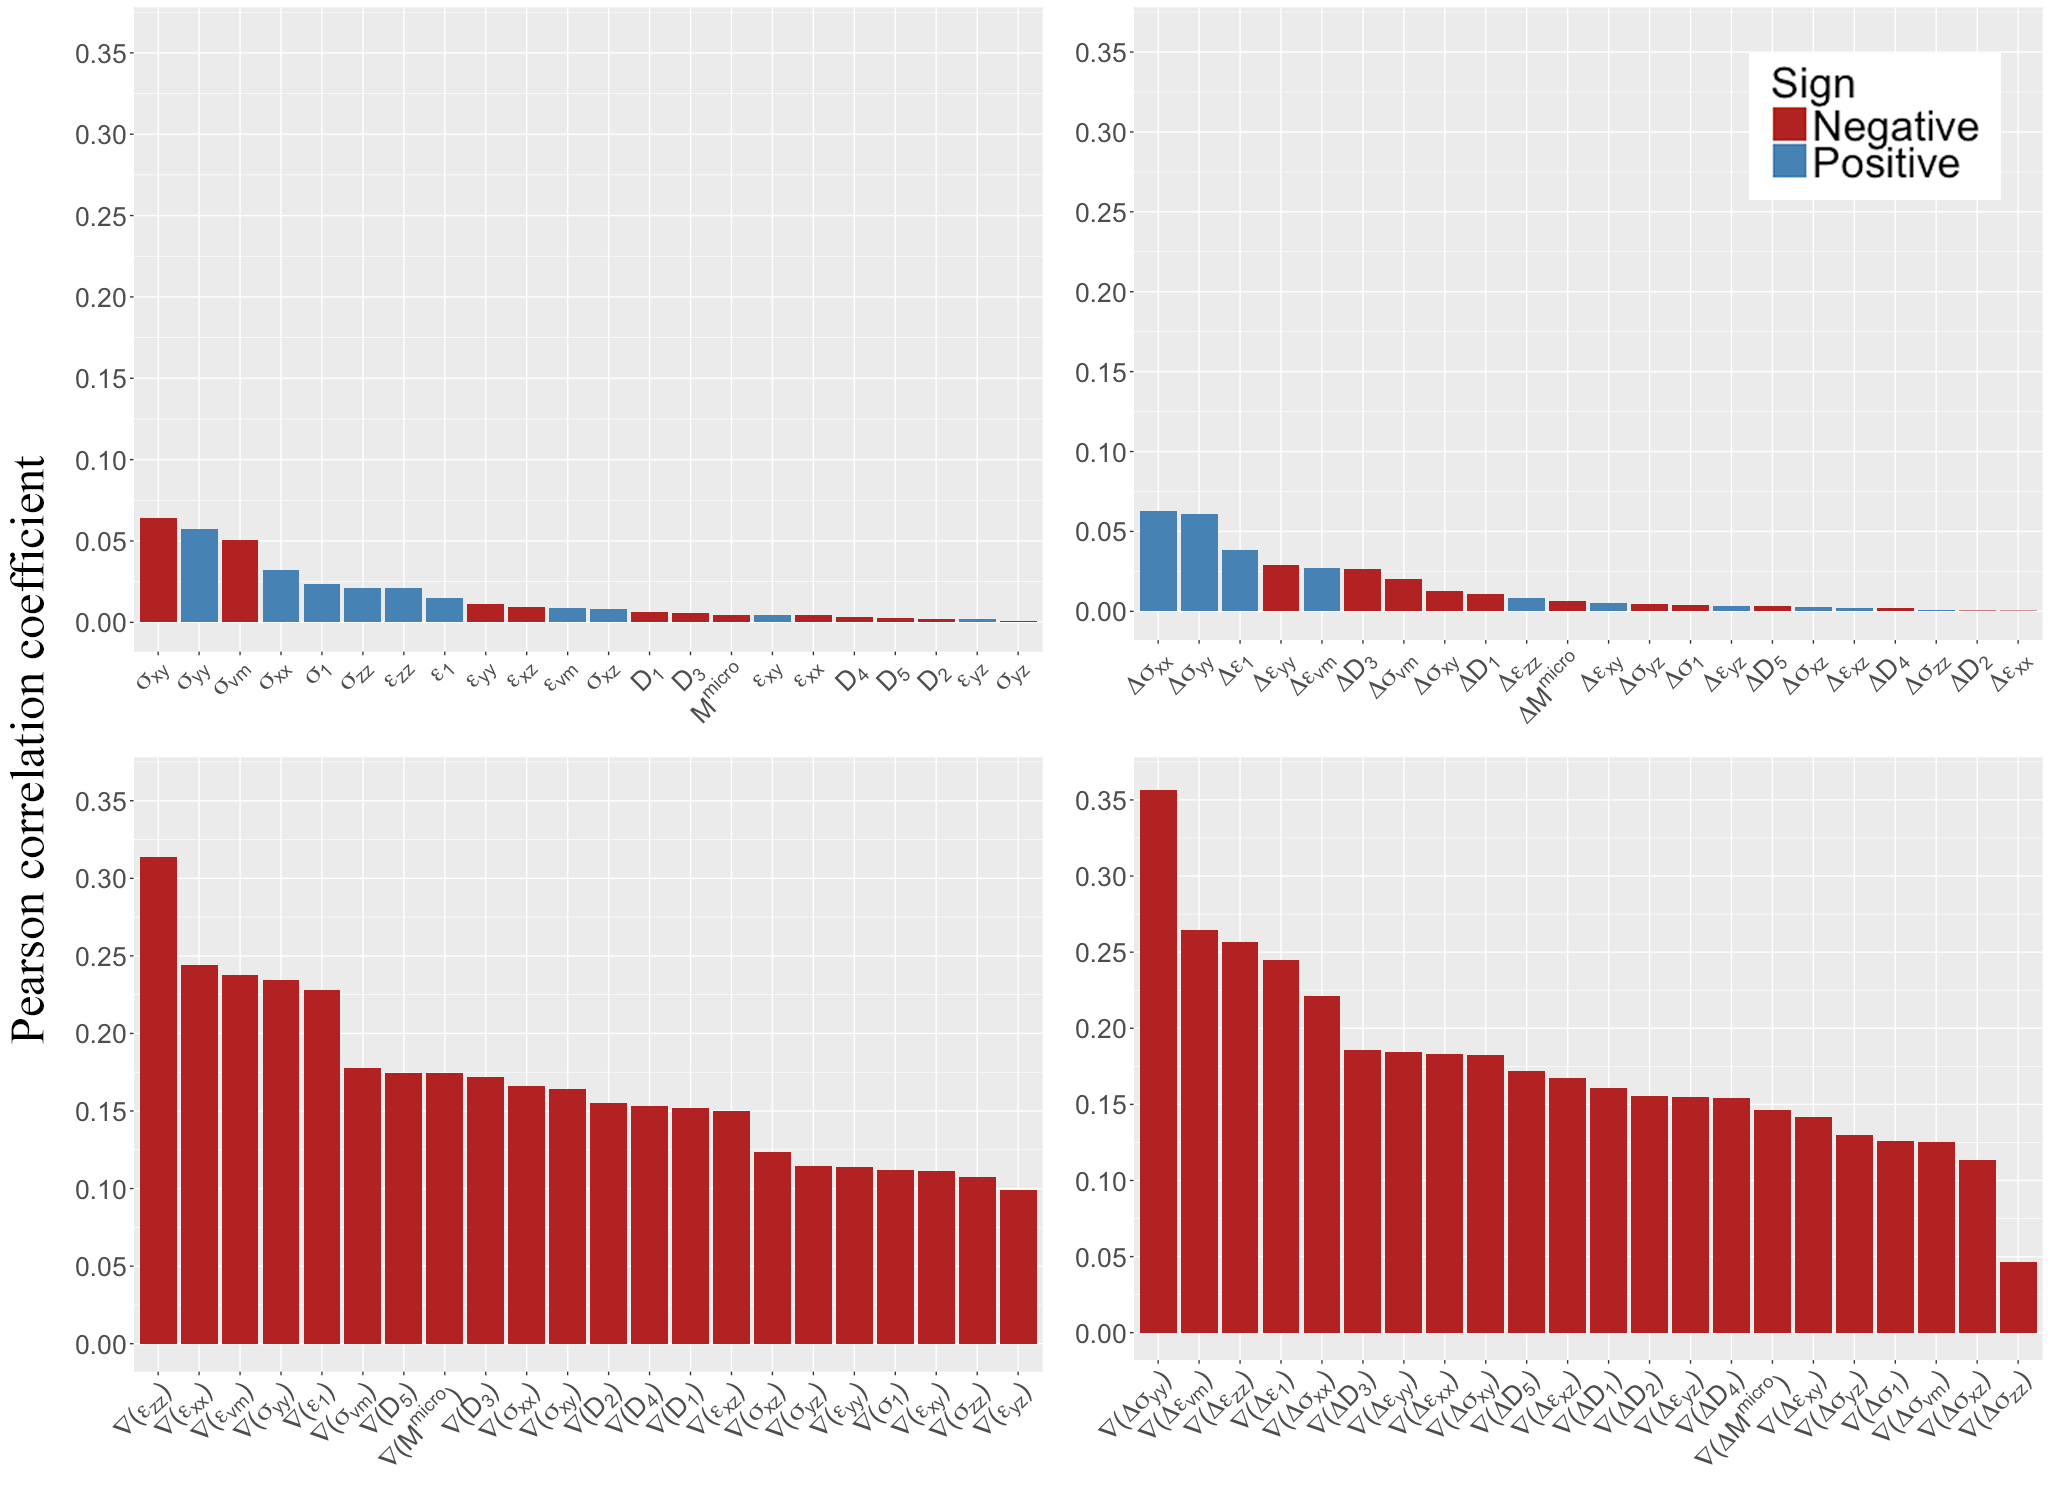
\includegraphics[width=\hsize]{correlations}
    \caption{Correlation coefficients computed between the following metrics and distance to crack surface: (a) field variables, $\lambda$; (b) cyclic change in field variables, $\Delta\lambda$; (c) spatial gradient of field variables, $\nabla(\lambda)$; (d) spatial gradient of cyclic field variables, $\nabla(\Delta\lambda)$.}
    \label{fig:correlations}
\end{figure}

The correlation coefficients shown in Fig.~\ref{fig:correlations} are not, at first look, overwhelmingly high. The challenge in assessing the statistical significance of these correlations is that the independent and identically distributed assumption required by a typical t-test has been violated. A nonparametric measure, such as bootstrapping \cite{good2010} or using Spearman rank, could potentially help resolve this problem. An alternative approach to determine whether the correlation values in Fig.~\ref{fig:correlations} are meaningful (but not necessarily statistically significant) is to apply the same correlation algorithm to alternative surfaces that could serve as hypothetical crack paths through the microstructure. Four alternative paths are considered: two z-normal planes positioned 200 $\mu m$ above and below the lower and upper faces, respectively, of the microstructural domain, and two instances of the measured crack surface offset by 125 $\mu m$ above and below the known crack path. Fig.~\ref{fig:correlations_offset_surfaces} shows the results for the latter two cases. Results for the two z-normal planes are provided in Fig. ~\ref{fig:correlations_offset_planes}. In all four cases, the correlations are consistently weaker than those for the actual crack surface, providing some evidence that micromechanical fields from a cyclically loaded, uncracked microstructure tend to correlate with the actual path of the 3D fatigue crack.

\begin{figure}[p]
  \centering
    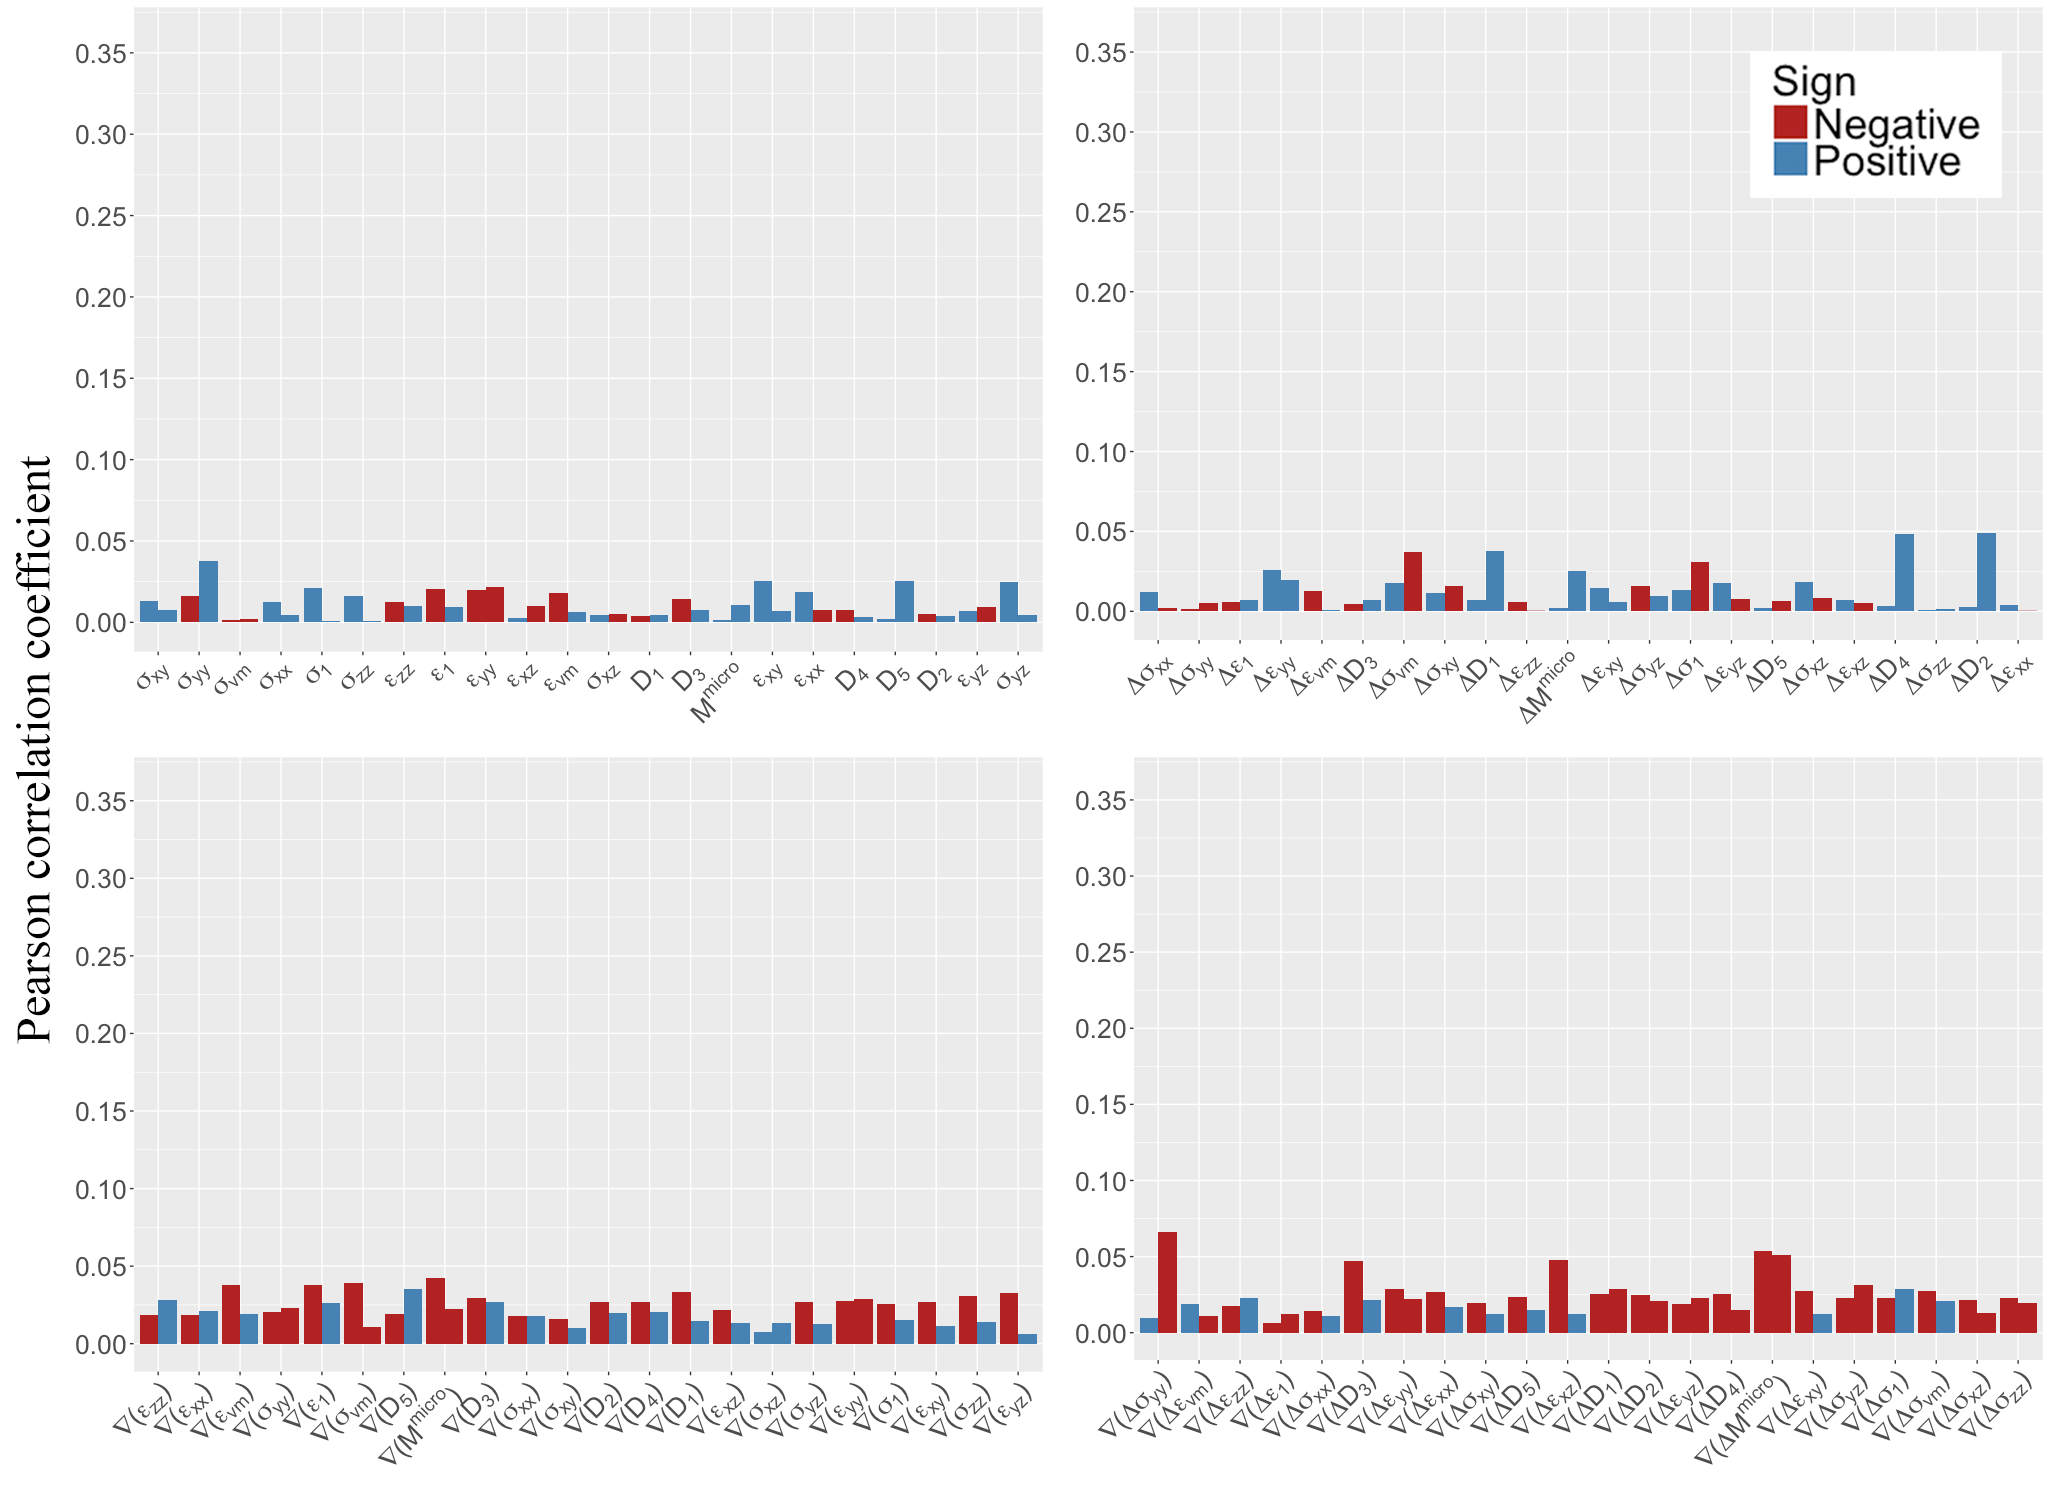
\includegraphics[width=\hsize]{correlations_offset_surfaces}
    \caption{Correlation coefficients computed between the following metrics and distance to hypothetical crack surfaces located 125 $\mu m$ below (left bars) and 125 $\mu m$ above (right bars) the known crack surface: (a) field variables, $\lambda$; (b) cyclic change in field variables, $\Delta\lambda$; (c) spatial gradient of field variables, $\nabla(\lambda)$; (d) spatial gradient of cyclic field variables, $\nabla(\Delta\lambda)$.}
    \label{fig:correlations_offset_surfaces}
\end{figure}

\begin{figure}[p]
  \centering
    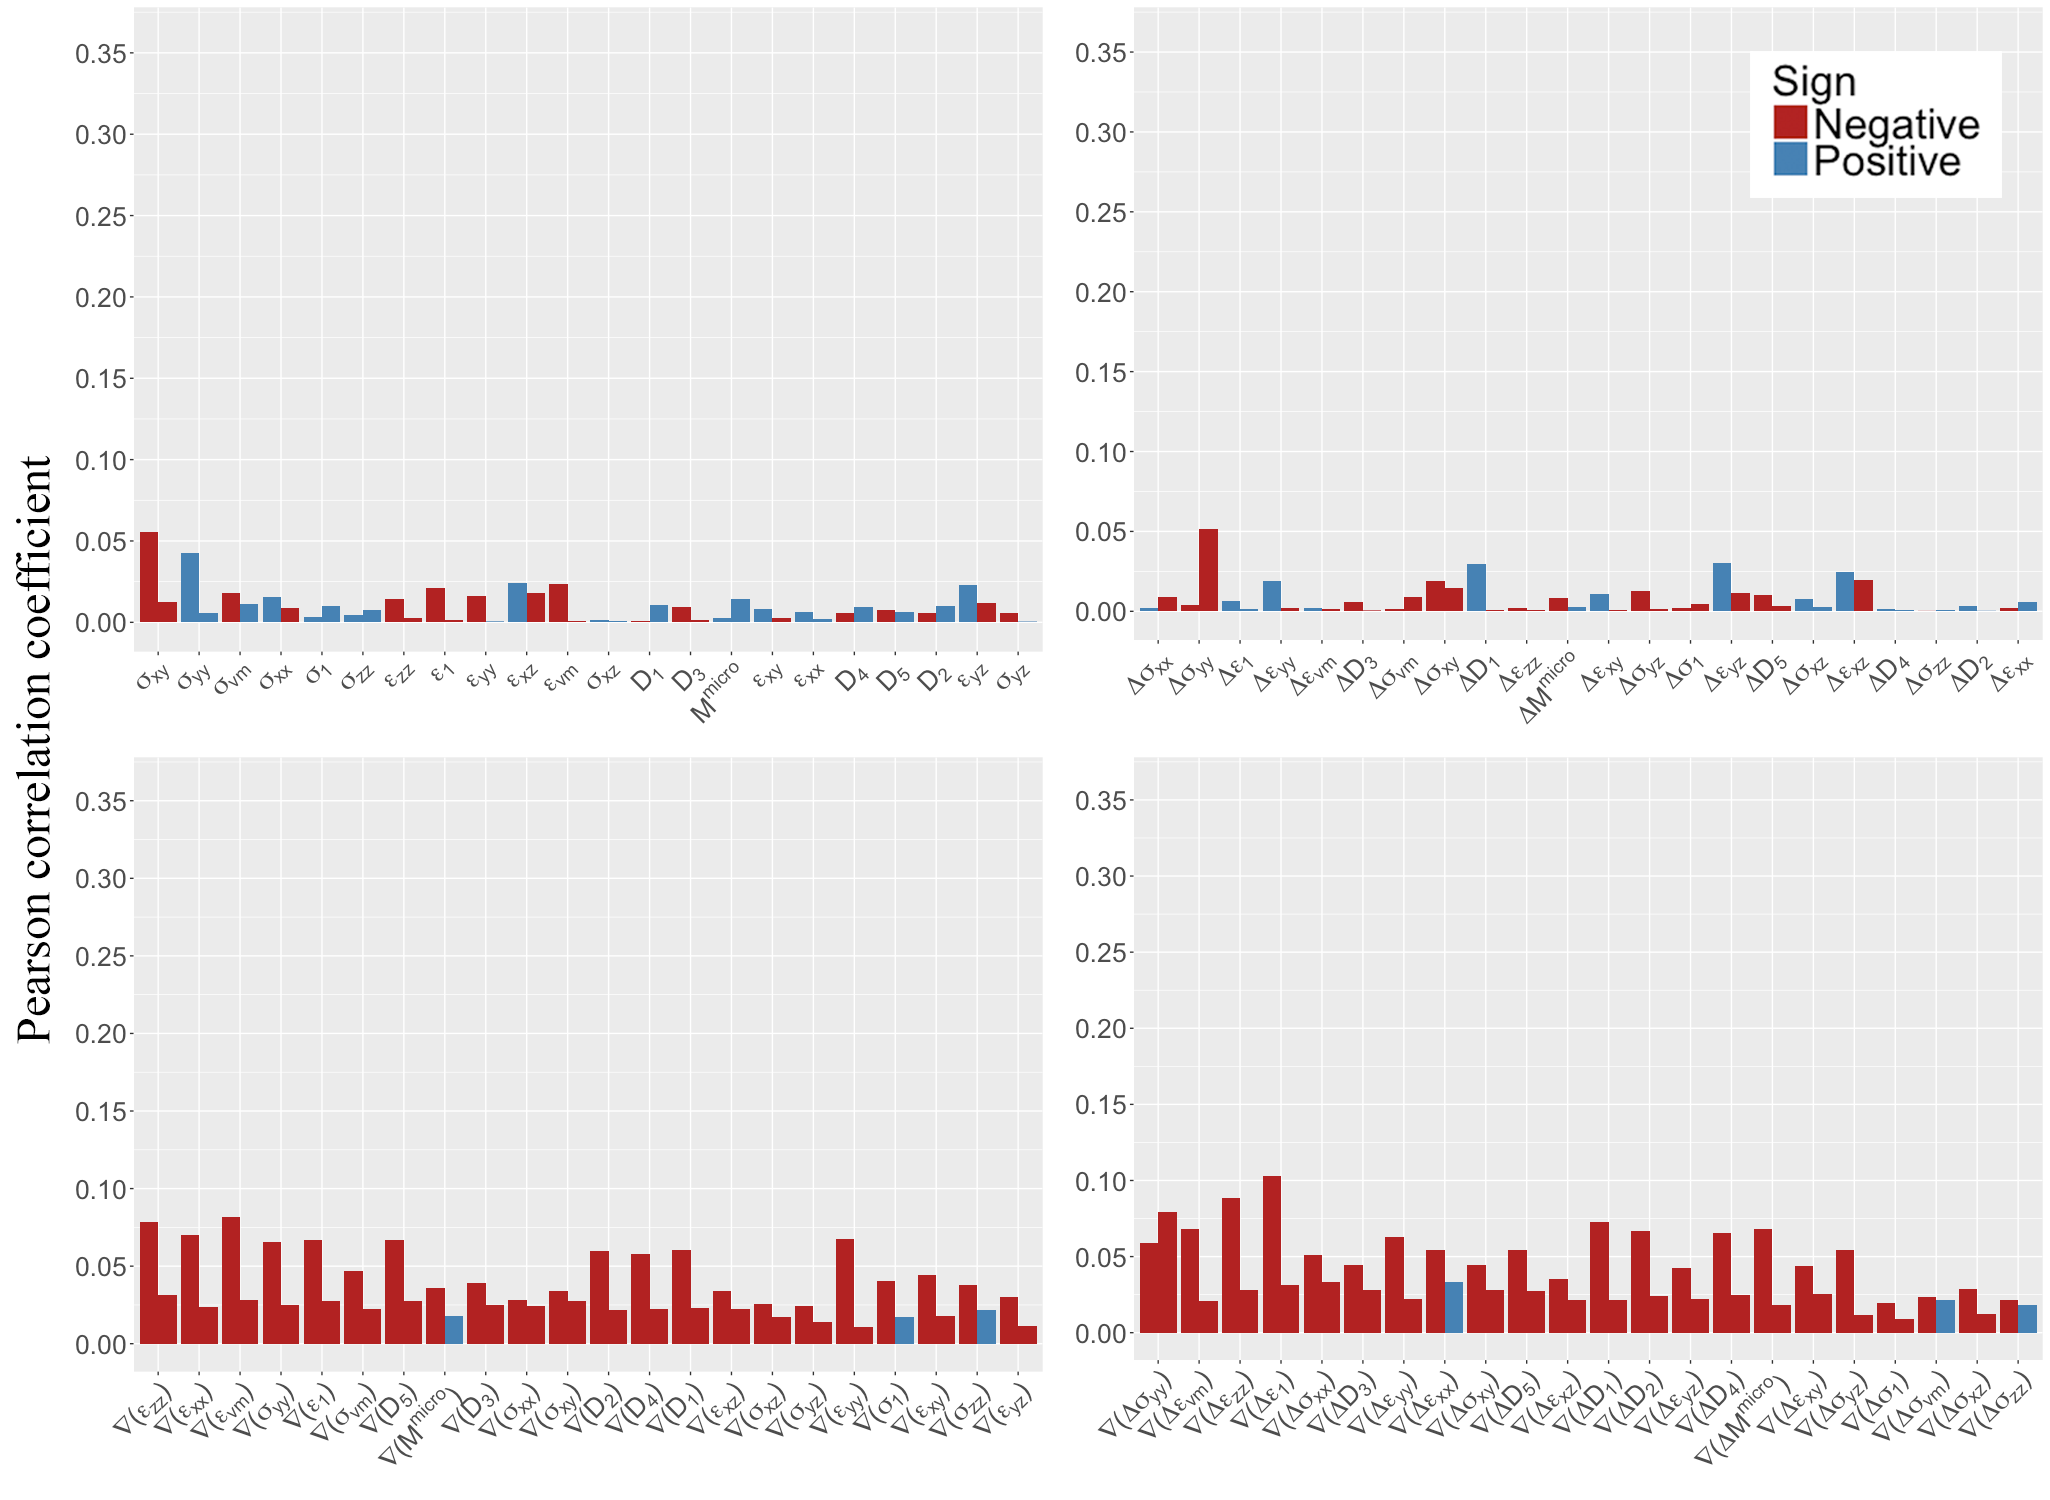
\includegraphics[width=\hsize]{correlations_offset_planes}
    \caption{Correlation coefficients computed between each variable and distance to z-normal planes located 200 $\mu m$ above the bottom face (left bars) and 200 $\mu m$ below the top face (right bars) of the microstructural domain.}
    \label{fig:correlations_offset_planes}
\end{figure}

As shown in Fig.~\ref{fig:correlations}, the crack path is generally shown to be more strongly correlated with the spatial-gradient values than with the field variables at peak load or with the cyclic field variables, suggesting that the eventual fatigue crack sought paths of high gradients in stress and/or strain space. Considering only the gradient-based parameters, $D_3$ and $D_5$ exhibit the strongest correlation with crack path among all slip-based damage metrics, although the difference is relatively marginal. This indicates that the combined effect of slip activity on multiple slip systems ($D_3$) as well as the combined effect of crystallographic slip and tensile stress on a slip plane ($D_5$) play a more significant role in predicting crack path than just the maximum value of slip on a single slip system or slip plane. While it seems reasonable for some of the metrics to have a relatively strong correlation with crack path (e.g.~$\nabla(\epsilon_{zz})$, $\nabla(\Delta\epsilon_{vm})$, and $\nabla(\Delta\epsilon_{1})$), there are other correlations that are not immediately intuitive (e.g.~$\nabla(\epsilon_{xx})$ and $\nabla(\Delta\sigma_{yy})$). Clearly, the factors affecting crack growth are highly complex, and we cannot rely on treating all field variables as independent mechanisms. As such, it is likely that there exists some complex combination of variables that serves to accommodate, promote, or hinder crack propagation, which corroborates previous conclusions in the literature (e.g.~\cite{McDowell_2010,Hochhalter_2011,Rovinelli_2017}). It will require further investigation using, for example, machine learning to understand how interaction of the variables leads to such apparent correlations. 

Since the discontinuity of the crack is not modeled in this work (as was done in previous work \cite{spear2016}), the micromechanical fields computed here do not account for stress redistribution due the formation of new traction-free surface area; nor do they account for plastic zones or stress concentrations in the vicinity of a crack front. However, the objective is to identify what, if any, correlations exist between micromechanical fields in an uncracked microstructure and the 3D path of an eventual fatigue-crack surface. The implications of relatively strong correlations could be significant, in that the crack path might be approximated prior to (or without having to) incorporate geometrically explicit crack representations. It is expected that such correlations would be relatively strong within a limited spatial domain surrounding the crack-nucleation site. Future work could investigate the size of this domain, beyond which the correlations are expected to diminish. 

The analysis from this work could provide insight into the extraction of relevant features for predictive machine-learning models. In models where univariate feature selection is required, such as convolution-based networks that infer useful information based on a grid of scalars, choosing the correct variables to use as a representation is critical. With new insight from the correlation analysis presented here, ongoing studies by the authors focus on the use of machine learning to identify critical combinations of, and relationships among, the most correlated variables with the evolution of fatigue-crack surfaces.

\section{Conclusions}
This work presents a systematic, data-driven approach to parameterize and correlate local micromechanical fields computed for an uncracked, cyclically loaded specimen with the known 3D fatigue-crack path observed from experiment. Specifically, local micromechanical field variables in the vicinity of an eventual crack surface are correlated with distance to that eventual surface. The intent is to identify whether the response of the uncracked microstructure subjected to realistic far-field loading might provide any predictive power in identifying the path of a fatigue-failure surface, which could have implications for future modeling efforts. In this work, a total of 88 micromechanical parameters, and $1.264\times 10^{9}$ data points, are considered in the analysis. Thus, the data used here are considered to be large and rich in nature, albeit for just a single specimen. The parameters include field variables and slip-based damage metrics computed at peak load, as well as their corresponding cyclic values. Also considered are the gradients of all previously mentioned parameters. The micromechanical parameters, taken at discrete points, are then correlated with the distance from a given point to the known crack surface. 

In general, the gradients of the micromechanical field variables appear to exhibit a stronger correlation with crack path than the field variables, themselves. This supports the claim that fatigue cracks generally seek paths of high gradients of stress, strain, or both. The variables, treated independently, are not sufficient to fully describe evolution of fatigue-crack surfaces. However, the systematic correlation analysis from this work provides insight into the extraction of relevant features for future development and testing of predictive models.

\section{Acknowledgements}
This material is based on research sponsored by the Air Force Office of Scientific Research Young Investigator Program, under agreement number FA9550-15-1-0172. The authors gratefully acknowledge Drs.~Ravi Chona, Ben Smarslok, and Brian Gockel of the Air Force Research Laboratory for their support of the work. The support and resources from the Center for High Performance Computing at the University of Utah are gratefully acknowledged.

\bibliographystyle{ieeetr}
\bibliography{\jobname}
